\documentclass{article}
\usepackage[utf8]{inputenc}
\usepackage{mathtools, amssymb, amsthm}
\usepackage{fullpage}
\usepackage{physics}
\usepackage{siunitx}
\usepackage{comment}
\usepackage{subcaption}
\usepackage[draft]{graphicx}

\usepackage{tikz}
\usetikzlibrary{arrows}

\usepackage[
    pdfusetitle,
    colorlinks
]{hyperref}

\usepackage[
    backend=biber,
    style=numeric,
    sorting=none,
    maxbibnames=99, minbibnames=99,
    natbib=true,
    url=false,
    eprint=true,
    pagetracker,
    giveninits]{biblatex}
\bibliography{slm}

\title{Multi-Scale Multi-Physics Modeling and Simulation of Selective Laser Melting}
\date{\today}
\author{O.A.~Rogozin, E.L.~Sharaborin, A.V.~Vezolainen, O.V.~Vasilyev}

\newcommand{\dder}[2][]{\Delta_{#2}#1}
\newcommand{\transpose}[1]{#1^\mathsf{T}}
\newcommand{\diag}[1]{\qty(#1)^\mathrm{diag}}
\newcommand{\fusion}[1]{{#1}^\mathrm{fus}}

% dimensionless variables
\newcommand{\Hx}{\hat{x}}
\newcommand{\Ht}{\hat{t}}
\newcommand{\Hh}{\hat{h}}
\newcommand{\HT}{\hat{T}}
\newcommand{\HP}{\hat{P}}
\newcommand{\Halpha}{\hat{\alpha}}
\newcommand{\Hsigma}{\hat{\sigma}}
\newcommand{\Hf}{\hat{f}}
\newcommand{\Hc}{\hat{c}}
\newcommand{\Hk}{\hat{k}}
\newcommand{\Hphi}{\hat{\phi}}
\newcommand{\Hpsi}{\hat{\psi}}
\newcommand{\HR}{\hat{R}}
\newcommand{\HU}{\hat{U}}
\newcommand{\HL}{\hat{L}}

\newcommand\OVV[1]{{\color{magenta}#1}}
\newcommand\OVVl[1]{{\color{magenta}$\leftarrow$[{\em #1}]}}
\newcommand\OVVr[1]{{\color{magenta} [{\em #1}]$\rightarrow$}}

\begin{document}
\maketitle
\tableofcontents

\section{Formulation of the problem}

%%% The first law of thermodynamics
The conservation of energy for a substance at rest is described by the \(D\)-dimensional heat-conduction equation
\begin{equation}\label{eq:heat_conduction}
    \rho\pdv{h(T)}{t} = \pdv{x_i}\qty( k(\psi,T)\pdv{T}{x_i} ),
\end{equation}
where \(x_i\) are the physical coordinates (\si{m}), \(t\) is the time (\si{s}),
\(\rho\) is the density (\si{kg/m}\(^D\)), \(h\) is the specific enthalpy (\si{J/kg}),
\(T\) is the temperature (\si{\K}), \(k\) is the thermal conductivity (\si{W/Km}\(^{D-2}\)),
\(\psi\) is the porosity, and the Einstein notation is assumed. Let
\begin{equation}\label{eq:porosity_variables}
    \rho = \rho_0(1-\psi_0), \quad k = k_0(T)(1-\psi),
\end{equation}
where \(\rho_0\) and \(k_0\) are the density and thermal conductivity of the bulk material, respectively,
and \(\psi_0\) is the initial porosity.

%%% Introduce a liquid fraction
To incorporate the fusion process into the model, the following dependance of \(h\) on \(T\) is assumed:
\begin{equation}\label{eq:enthalpy}
    h = \int_{T_0}^T c_p(\xi)\dd{\xi} + \fusion{h}\phi(h),
\end{equation}
where \(c_p\) is the specific heat capacity (\si{J/kgK}), \(\fusion{h}\) is the specific enthalpy of fusion (\si{J/kg}),
\(\phi\) is the liquid fraction (\(0 \leq \phi \leq 1\)).
The limits \(\phi=0\) and \(\phi=1\) correspond to the solid and liquid states, respectively.
Substituting Eqs.~\eqref{eq:porosity_variables} and~\eqref{eq:enthalpy} into Eq.~\eqref{eq:heat_conduction},
the governing equation for \(h\) becomes
\begin{equation}\label{eq:heat_conduction2}
    \rho_0\pdv{h}{t} = \pdv{x_i}\qty( \frac{1-\psi}{1-\psi_0} \frac{k_0(T)}{c_p(T)}\pdv{h_*}{x_i} ),
\end{equation}
where \(h_* = h - \fusion{h}\phi\) is introduced for convenience.

%%% Change in thermophysical properties resulting from fusion process
The phase transition results in an abrupt change in the thermophysical properties \(f=c_p,k_0\) of the material;
therefore, they can be expressed as
\begin{equation}\label{eq:fusion_change}
    f = f_S(T) + \qty( f_L(T) - f_S(T) )\phi,
\end{equation}
where \(f_S\) and \(f_L\) correspond to solid and liquid properties.
The porosity change is irreversible in time:
\begin{equation}\label{eq:porosity}
    \psi(t) = \psi_0\min_{0\leq\tau\leq t}\qty( 1-\phi(h(\tau)) ).
\end{equation}

%%% Initial and boundary conditions
Let us consider a half-space problem \(x_D<0\) with the following boundary condition at \(x_D=0\):
\begin{equation}\label{eq:bc}
    k(\psi,T)\pdv{T}{x_D} = \frac{A(\psi)P}{(\pi R^2)^{(D-1)/2}}\exp\qty( -\sum_{i\neq D}\frac{\qty[x_i-x_{Bi}(t)]^2}{R^2} )
        - \alpha(T-T_0) - \epsilon\sigma T^{D+1},
\end{equation}
where \(A\) is the absorptivity, \(P\) is the laser power (\si{W}), \(R\) is the radius of the laser beam (\si{m}),
\(x_{Bi}\) are the coordinates of its center (\si{m}), \(\alpha\) is the convective heat transfer coefficient (\si{W/Km}\(^{D-1}\)),
\(\epsilon\) is the emissivity, \(\sigma\) is the Stefan--Boltzmann constant (\si{W/K}\(^{D+1}\)\si{m}\(^{D-1}\)).
The initial condition at \(t=0\) is \(T=T_0\), \(\Hpsi = \psi_0\) and \(\Hpsi = 0\) for the powder and solid states, respectively.

\subsection{Dimensionless expressions}

In the present study, the variables are dimensionalized as follows:
\begin{equation}\label{eq:dimensionless}
    \begin{aligned}
        x_i &= \Hx_iR, & t &= \Ht t_0, & h &= \Hh c_p(T_0)\Delta{T}, & T - T_0 &= \HT\Delta{T}, \\
        P &= \HP k_0(T_0)\Delta{T}R^{D-2}, & \alpha &= \Halpha\frac{k_0(T_0)}R, &
            \sigma &= \Hsigma\frac{k_0(T_0)}{R\Delta{T}^D}, & T_0 &= \HT_0\Delta{T}, \\
    \end{aligned}
\end{equation}
where \(t_0 = \rho_0 c_p(T_0) R^2/k_0(T_0)\) is the diffusive time scale at \(T=T_0\),
\(\Delta{T} = (T_S+T_L)/2 - T_0\) is the unit temperature,
\(T_S\) and \(T_L\) are the solidus and liquidus temperatures, respectively.
If \(|\pdv*{x_{Bi}}{t}|\) is of order \(U_0\), where \(U_0\) is the reference scanning speed (\si{m/s}),
then \(R/U_0=t_0/\HU_0\) is the convective time scale. Also denote
\begin{equation}\label{eq:dimensionless2}
    \Hc_p(\HT) = \frac{c_p(T)}{c_p(T_0)}, \quad
    \Hk_0(\HT) = \frac{k_0(T)}{k_0(T_0)}, \quad
    \Hphi(\Hh) = \phi(h), \quad
    \Hpsi(\Hh) = \psi(h).
\end{equation}
Then~\eqref{eq:enthalpy},~\eqref{eq:heat_conduction2},~\eqref{eq:porosity} and~\eqref{eq:bc} take the following nondimensional form:
\begin{gather}
    \Hh_* \equiv \Hh - \fusion{\Hh}\Hphi = \int_0^{\HT} \Hc_p(\xi)\dd{\xi}, \label{eq:enthalpy_hats} \\
    \pdv{\Hh}{\Ht} = \pdv{\Hx_i}\qty(
        \frac{1-\Hpsi}{1-\psi_0}
        \frac{\Hk_0(\HT)}{\Hc_p(\HT)}\pdv{\Hh_*}{\Hx_i}
    ), \label{eq:heat_conduction_hats} \\
    \Hpsi(\Ht) = \psi_0\min_{0\leq\tau\leq \Ht}\qty( 1-\Hphi(\Hh(\tau)) ), \label{eq:porosity_hats} \\
    \qty(1 - \Hpsi) \frac{\Hk_0(\HT)}{\Hc_p(\HT)}\pdv{\Hh_*}{\Hx_D} +
        \Halpha\HT + \epsilon\Hsigma \qty(\HT + \HT_0)^{D+1} =
        \frac{A(\Hpsi)\HP}{\pi^{(D-1)/2}}\exp\qty( -\sum_{i\neq D}\qty[\Hx_i-\Hx_{Bi}(t)]^2 ). \label{eq:bc_hats}
\end{gather}
The initial condition is \(\Hh = 0\).

\subsection{Thermophysical properties}

For conventional materials, the required thermophysical properties can be reasonably approximated
by the three-parameter model (Fig.~\ref{fig:thermophysical})
\begin{equation}\label{eq:thermophysical_model}
    \Hf = 1 + \Hf'_S\HT + \qty[
        \fusion{\Hf} + \qty(\Hf'_L-\Hf'_S) \qty(\HT-1)
    ]\Hphi,
\end{equation}
where \(\Hf'_{S,L}\) are the corresponding constant first temperature derivatives far from fusion process,
\(\fusion{\Hf}\) is the property jump at the phase transition.
Matching~\eqref{eq:thermophysical_model} with~\eqref{eq:fusion_change}, we obtain
\begin{equation}\label{eq:thermophysical_model_explicit}
    \Hf_S = 1 + \Hf'_S\HT, \quad
    \Hf_L = \Hf_{L0} + \Hf'_L\HT,
\end{equation}
where \(\Hf_{L0} = 1 + \Hf'_S - \Hf'_L + \fusion{\Hf}\).

\begin{figure}
    \centering
    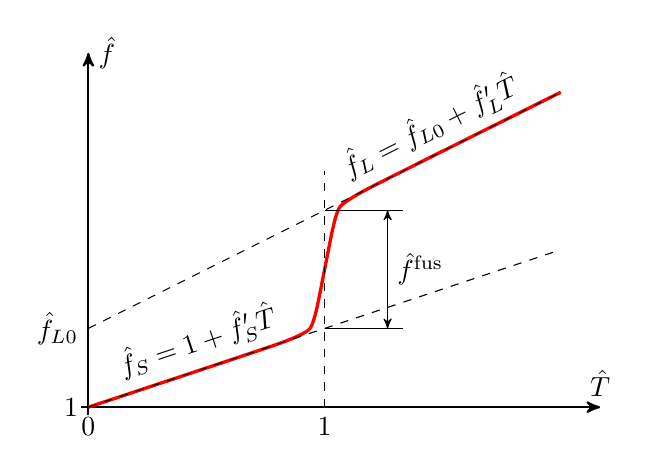
\begin{tikzpicture}[thick, >=stealth']
        \coordinate (O) at (0,0);
        \draw[->] (-0.1,0) -- (6.5,0) node[above] {$\HT$};
        \draw[->] (0,-0.1) -- (0,4.5) node[right] {$\Hf$};

        \path (O) -- (3,1) node[midway,sloped,above] {$\Hf_S=1+\Hf'_S\HT$}
            -- (3,2.5) -- (6,4) node[midway,sloped,above] {$\Hf_L=\Hf_{L0}+\Hf'_L\HT$};
        \draw[red, very thick] plot[smooth,tension=0.3,mark=] coordinates{
            (0,0) (2.4,2.4/3) (2.8, 2.8/3+0.05) (2.9,3.5/2-0.5) (3.1,3.5/2+0.5) (3.2,2.5+0.2/2-0.05) (3.6,2.5+0.6/2) (6,4)};
        \draw[thin,dashed] (0,1) coordinate(A) -- (6,4);
        \draw[thin,dashed] (O) -- (6,2);
        \draw[thin,dashed] (3,0) coordinate(F) -- (3,3);

        \node[below] at (O) {$0$};
        \node[below] at (F) {$1$};
        \node[left] at (O) {$1$};
        \node[left] at (A) {$\Hf_{L0}$};

        \draw[thin] (3,1) -- (4,1);
        \draw[thin] (3,2.5) -- (4,2.5);
        \draw[thin,<->] (3.8,1) -- (3.8,2.5) node[midway,right] {$\fusion{\Hf}$};
    \end{tikzpicture}
    \caption{Dimensionless thermophysical properties versus temperature for the three-parameter model~\eqref{eq:thermophysical_model}.}
    \label{fig:thermophysical}
\end{figure}

\subsection{Temperature evaluation}

%%% 5-parameter model
For arbitrary \(\Hphi(\Hh)\), solution of~\eqref{eq:enthalpy_hats} is not straightforward.
However, the temperature is included in~\eqref{eq:heat_conduction_hats} and~\eqref{eq:bc_hats}
only through thermophysical properties and, therefore, can be evaluated approximately.
Several approaches can be employed to work around this difficulty.
We employ the \(\Hphi\)-based approximation~\eqref{eq:fusion_change} based on the five-parameter model:
\begin{equation}\label{eq:enthalpy_phi}
    \Hh = \Hh'_S\HT + \frac{\Hh''_S}2\HT^2 + \qty[
        \fusion{\Hh} + \qty(\Hh'_L-\Hh'_S) \qty(\HT-1) + \frac{\Hh''_L-\Hh''_S}2 \qty( \HT^2-1 )
    ]\Hphi,
\end{equation}
where
\begin{equation}\label{eq:enthalpy_phi_params}
    \Hh'_S = 1, \quad \Hh'_L = 1 + \Hc'_{pS} - \Hc'_{pL} + \fusion{\Hc}_p, \quad
    \Hh''_S = \Hc'_{pS}, \quad \Hh''_L = \Hc'_{pL}
\end{equation}
should be satisfied for~\eqref{eq:enthalpy_phi} to be consistent with \(\Hc_p(\HT)\)
defined by~\eqref{eq:thermophysical_model}.
Indeed,~\eqref{eq:enthalpy_phi_params} results from the following assumption:
\begin{equation}\label{eq:enthalpy_phi_explicit}
    \eval{\Hh}_{\Hphi=0} = \Hh_S(\HT) \equiv \int_0^{\HT} \Hc_{pS}(\xi)\dd{\xi}, \quad
    \eval{\Hh}_{\Hphi=1} = \Hh_L(\HT) \equiv \Hh_S(1) + \fusion{\Hh} + \int_1^{\HT} \Hc_{pL}(\xi)\dd{\xi},
\end{equation}
where \(\Hc_{pS,L}\) is defined as~\eqref{eq:thermophysical_model_explicit}.

%%% Explicit formulas for temperature
Actually,~\eqref{eq:enthalpy_phi} is the quadratic equation with respect to \(\HT\), hence
\begin{equation}\label{eq:temp_phi}
    \HT = \frac{\sqrt{g_1^2 + 2g_2g_3}-g_1}{g_2}, \quad
    \dv{\HT}{\Hh} = \frac{g_3' - g_1'\HT - \frac12g_2'\HT^2}{g_2\HT + g_1},
\end{equation}
where
\begin{equation}\label{eq:enthalpy3_phi}
    g_{1,2}(\Hh) = \Hh_S^{\prime,\prime\prime} (1-\Hphi) + \Hh_L^{\prime,\prime\prime}\Hphi, \quad
    g_3(\Hh) = \Hh_* + \qty(\Hh_L' - \Hh_S' + \frac{\Hh_L'' - \Hh_S''}2)\Hphi.
\end{equation}

\subsection{Liquid fraction models}

%%% Requirements
Denote \(\Hh_1 = \Hh(1)\), \(\Hphi'_1 = \Hphi'(\Hh_1)\) and
impose the following requirements upon \(\Hphi(\Hh)\):
\begin{gather}
    \Hphi'_1 = \frac1{\Hh_L(\HT_L)-\Hh_S(\HT_S)}, \label{eq:lf_derivative}\\
    0 \leq \Hphi' \leq \Hphi'_1, \label{eq:lf_monotonic}\\
    \Hphi(\Hh_1 - \Hh) = 1-\Hphi(\Hh) \quad (\Hh\geq\Hh_1), \label{eq:lf_symmetric}\\
    \begin{cases}
        \phi(\Hh) = \order{(\Hh_1-\Hh)^{-\infty}} \quad (\Hh < \Hh_1), \\
        \phi(\Hh) = 1+\order{(\Hh-\Hh_1)^{-\infty}} \quad (\Hh > \Hh_1).
    \end{cases}\label{eq:lf_exp_decay}
\end{gather}
Thickness of the solid--liquid interface is defined by~\eqref{eq:lf_derivative},
inequalities~\eqref{eq:lf_monotonic} are the monotonic condition and boundedness of the fusion rate,
\eqref{eq:lf_symmetric} is the symmetric property,
and~\eqref{eq:lf_exp_decay} describes fast decay of \(\Hphi(\Hh)\) outside the fusion range.
Note that \(\Hphi_1 = \Hphi(\Hh_1) = 1/2\).

%%% Examples of \Hphi'_1
The fixed value of \(\Hphi'_1\) depends only on \(\HT_{S,L}\), \(\Hc'_{pS,L}\), \(\fusion{\Hh}\), and \(\fusion{\Hc_p}\).
Incidentally, \(\Hphi'_1 = (\fusion{\Hh})^{-1}\) when \(\HT_S=\HT_L\)
and \(\Hphi'_1 = (\fusion{\Hh}+\delta\fusion{\HT})^{-1}\) for the constant specific heat capacity,
where \(\delta\fusion{\HT} = \HT_L - \HT_S\).

%%% Examples of liquid fraction models
The simplest \(\mathcal{C}^0\) model for \(\Hphi(\Hh)\) can be constructed as a piecewise approximation
\begin{equation}\label{eq:lf_piecewise}
    \Hphi = \begin{cases}
        0,                                            & \Hh \leq \Hh(\HT_S), \\
        \qty(\Hh-\Hh(\HT_S))\Hphi'_1, & \Hh(\HT_S) < \Hh < \Hh(\HT_L), \\
        1,                                            & \Hh(\HT_L) \leq \Hh.
    \end{cases}
\end{equation}
The hyperbolic tangent yields the \(\mathcal{C}^\infty\) model
\begin{equation}\label{eq:lf_tanh}
    \Hphi = \frac1{1+\exp\qty(-4\Hphi'_1(\Hh-\Hh_1))}.
\end{equation}

\subsection{Space and time scales}

It is possible to identify several space scales in the considered problem:
\begin{itemize}
    \item solid--liquid interface thickness \(\delta\fusion{\Hx}\),
    \item radius of the laser beam \(1\),
    \item length of the whole domain \(\HL\).
\end{itemize}

Let the local interface thickness be defined at isotherm \(\HT=1\) as
\begin{equation}\label{eq:thickness_def}
    \delta\fusion{\Hx} = \qty|\pdv{\Hphi}{\Hx_i}|^{-1}.
\end{equation}
It can be evaluated after substitution~\eqref{eq:lf_derivative} into the spatial derivative from~\eqref{eq:enthalpy_hats}, which gives
\begin{equation}\label{eq:thickness_general}
    \fusion{\delta\Hx} = \frac{1-\fusion{\Hh}\Hphi'_1}{\Hphi'_1\Hc_p(1)}\qty|\pdv{\HT}{\Hx_i}|^{-1}.
\end{equation}
For the constant specific heat capacity,
\begin{equation}\label{eq:thickness_const}
    \fusion{\delta\Hx} = \delta\fusion{\HT}\qty|\pdv{\HT}{\Hx_i}|^{-1}.
\end{equation}

There is also a set of time scales:
\begin{itemize}
    \item diffusive \(\Ht_\mathrm{diff} = 1\),
    \item convective \(\Ht_\mathrm{conv} = \HU_0^{-1}\),
    \item fusion \(\Ht_\mathrm{fus} = (1+\fusion{\Hh})/\HP\).
\end{itemize}
If the fusion time scale is less than the convective one, the melting pool is formed under the influence of the laser heat source.

\section{Numerical methods}

Parallel Adaptive Wavelet Collocation Method (PAWCM)~\cite{Vasilyev2015} is employed for numerical solution of the problem
in order to capture solid--liquid interface with high accuracy while preserving computational efficiency.

\subsection{Time-marching scheme}

Evolution equation \(\pdv*{h}{t}=\mathcal{F}(h)\) is solved by the linearized Crank--Nicolson time integration method.
The discretization of the right-hand side~\eqref{eq:heat_conduction_hats}
\begin{equation}\label{eq:rhs}
    \mathcal{F} = \dder{\Hx_i}\qty(a \dder[\Hh_*]{\Hx_i})
\end{equation}
is perturbed as
\begin{equation}\label{eq:Drhs}
    \var{\mathcal{F}} = \dder{\Hx_i}\qty[ a'\var{\Hh}\dder[\Hh_*]{\Hx_i} + a\dder[\var{\Hh_*}]{\Hx_i} ],
\end{equation}
where \(\dder{\Hx_i}\) is the finite-difference approximation of the gradient,
\begin{equation}\label{eq:a}
    a(h) = \frac{1-\Hpsi}{1-\psi_0}\frac{\Hk_0(\HT)}{\Hc_p(\HT)}
\end{equation}
is the thermal diffusivity.
The resulting linear system is solved by the BICGSTAB (Biconjugate Gradient Stabilized) algorithm.
To accelerate convergence, the preconditioning procedure based on the following diagonal term is used:
\begin{equation}\label{eq:Drhs_diag}
    \diag{\fdv{\mathcal{F}}{h}} = a'\diag{\dder{\Hx_i}} \dder[\Hh_*]{\Hx_i} +
        a\Hh'_*\diag{\dder{\Hx_i}\dder{\Hx_i}},
\end{equation}
where \(\diag{\mathcal{L}}\) is the diagonal part of finite-difference operator \(\mathcal{L}\).

The computational mesh is refined adaptively at every time step
according to the local interpolation error for \(a\), \(\Hphi\), and \(\HT\).

\subsection{Boundary conditions}

Linearization of the boundary condition~\eqref{eq:bc_hats} around \(\Hh\) leads to
\begin{equation}\label{eq:bc_linearized}
    \qty(b' + a\qty(1 - \psi_0) \Hh'_* \dder{\Hx_D})\var{\Hh} =
        \frac{A(\Hpsi)\HP}{\pi^{(D-1)/2}}\exp\qty( -\sum_{i\neq D}\qty(\Hx_i-\Hx_{Bi})^2 ) - b,
\end{equation}
where
\begin{equation}\label{eq:bc_Dirichlet_part}
    b(\Hh) = \Halpha\HT + \epsilon\Hsigma\qty(\HT + \HT_0)^{D+1}.
\end{equation}

\subsection{Porosity evaluation}

The porosity defined in~\eqref{eq:porosity_hats} can be evaluated as
\begin{equation}\label{eq:porosity_eval}
    \Hpsi_0 = \psi_0, \quad \Hpsi_n = \min\qty(\Hpsi_{n-1}, \psi_0(1-\Hphi_n)) \quad (n\in\mathbb{N}),
\end{equation}
where subscript \(n\) corresponds to the value at \(n\) time iteration.
Its first derivative
\begin{equation}\label{eq:Dporosity}
    \Hpsi' = -\psi_0\max\qty(0, \Hphi') \begin{cases}
        1, \quad \Hpsi = \psi_0(1-\Hphi), \\
        0, \quad \Hpsi < \psi_0(1-\Hphi)
    \end{cases}
\end{equation}
can be evaluated as
\begin{equation}\label{eq:Dporosity_eval}
    \Hpsi'_0 = 0, \quad \Hpsi'_n = -\psi_0\Hphi'_n \begin{cases}
        1, \quad \Hpsi_n < \Hpsi_{n-1}, \\
        0, \quad \Hpsi_n = \Hpsi_{n-1}
    \end{cases}\quad (n\in\mathbb{N}).
\end{equation}

\subsection{Initial conditions}

To reduce initial oscillations, the initial condition should be consistent with the boundary conditions.
It means that the initial condition should satisfy~\eqref{eq:bc_hats} at \(\Hx_D=0\)
and decay exponentially to zero as we approach other boundaries.
For instance, consider the following two-parameter model:
\begin{gather}
    \HT = \HT_p\exp\qty( -\sum_{i\neq D}\frac{\qty[\Hx_i-\Hx_{Bi}(0)]^2}{\HR_p^2} )
        \exp\qty(\lambda \Hx_D - \frac{\Hx_D^2}{\HR_p^2}), \label{eq:ic_hats}\\
    \lambda = \eval{ \frac{A(\Hpsi)\HP\exp\qty( -\sum_{i\neq D}\qty(\Hx_i-\Hx_{Bi})^2\qty(1-\HR_p^{-2}) )}
        {\pi^{(D-1)/2}\HT_p k_0(\HT)(1-\Hpsi)} }_{\Hx_D=0}, \label{eq:lambda}
\end{gather}
where arbitrary \(\HT_p\) and \(\HR_p\) correspond to the maximum temperature
and radius of the initial melting pool, respectively.
They can be chosen to mimic the near-steady state.
Convective and radiative heat transfers are neglected in~\eqref{eq:ic_hats}.
The initial condition for the enthalpy is calculated as a solution of nonlinear equation~\eqref{eq:enthalpy_phi}.

\section{Single-track formation}

In this section, formation of a single straight track from the only powder layer covering the solid substrate is investigated.
For this problem, the boundary and initial conditions are supplemented with the following relations:
\begin{gather}
    x_{Bi} = \transpose{\qty(U_0,0,0)}t, \label{eq:single:bc} \\
    \psi = \psi_0\begin{cases}
        1, \quad x_D \geq -H, \\
        0, \quad x_D < -H.
    \end{cases}\label{eq:single:ic}
\end{gather}
where \(H\) is the thickness of the powder layer.
\begin{equation}\label{eq:single:params}
    \psi_0 = 0.4, \quad A = 0.3, \quad \epsilon = 0.3,
\end{equation}
and the corresponding thermophysical properties are assumed for the SS316L powder.

\subsection{Two-dimensional problem}

\begin{figure}
    \centering
    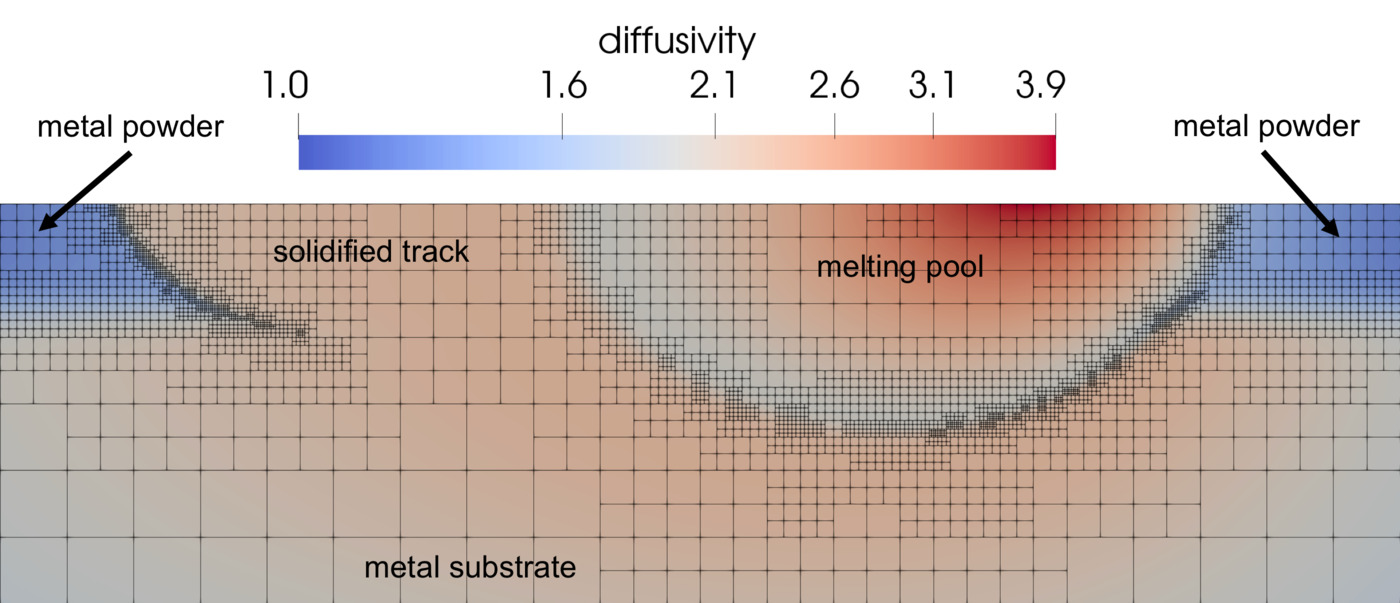
\includegraphics[width=\textwidth]{single_track/layer1_smooth2_mesh}
    \caption{
        The thermal diffusivity and computational mesh for the two-dimensional problem.
    }\label{fig:2d:mesh}
\end{figure}

\begin{figure}
    \centering
    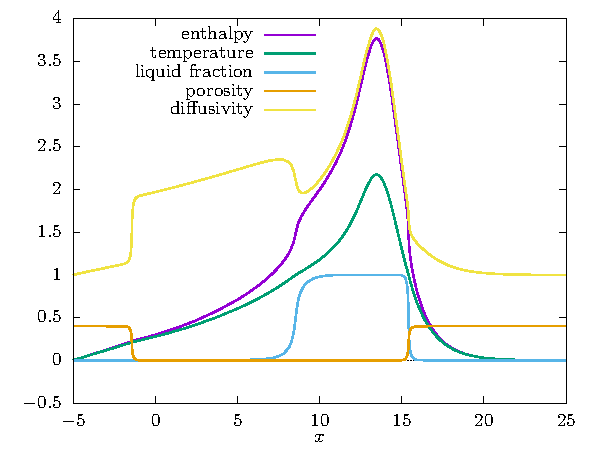
\includegraphics{single_track/layer1_smooth2}
    \caption{
        Profiles of the nondimensional quantities along the symmetry axis.
    }\label{fig:2d:profiles}
\end{figure}

From the computational point of view, the two-dimensional problem is much simpler than the three-dimensional one;
therefore, it is considered first of all in order to illustrate the proposed model.
Fig.~\ref{fig:2d:mesh} demonstrates how the computational mesh is effectively refined
to capture \(a\) with near-constant accuracy over the whole computational domain.
It is seen that the thermal diffusivity reaches its maximum in the point of the maximum temperature in the melting pool,
decreases rapidly as approaching the solid--liquid interface, jumps after solidification (typical for the stainless steel alloys),
and, finally, reduces to its minimum value in the powder region.
The profiles of the nondimensional quantities along \(x_1\) axis for \(x_D=0\) are shown in Fig.~\ref{fig:2d:profiles}.

\subsection{Three-dimensional problem}

\begin{figure}
    \centering
    \begin{subfigure}[b]{0.24\textwidth}
        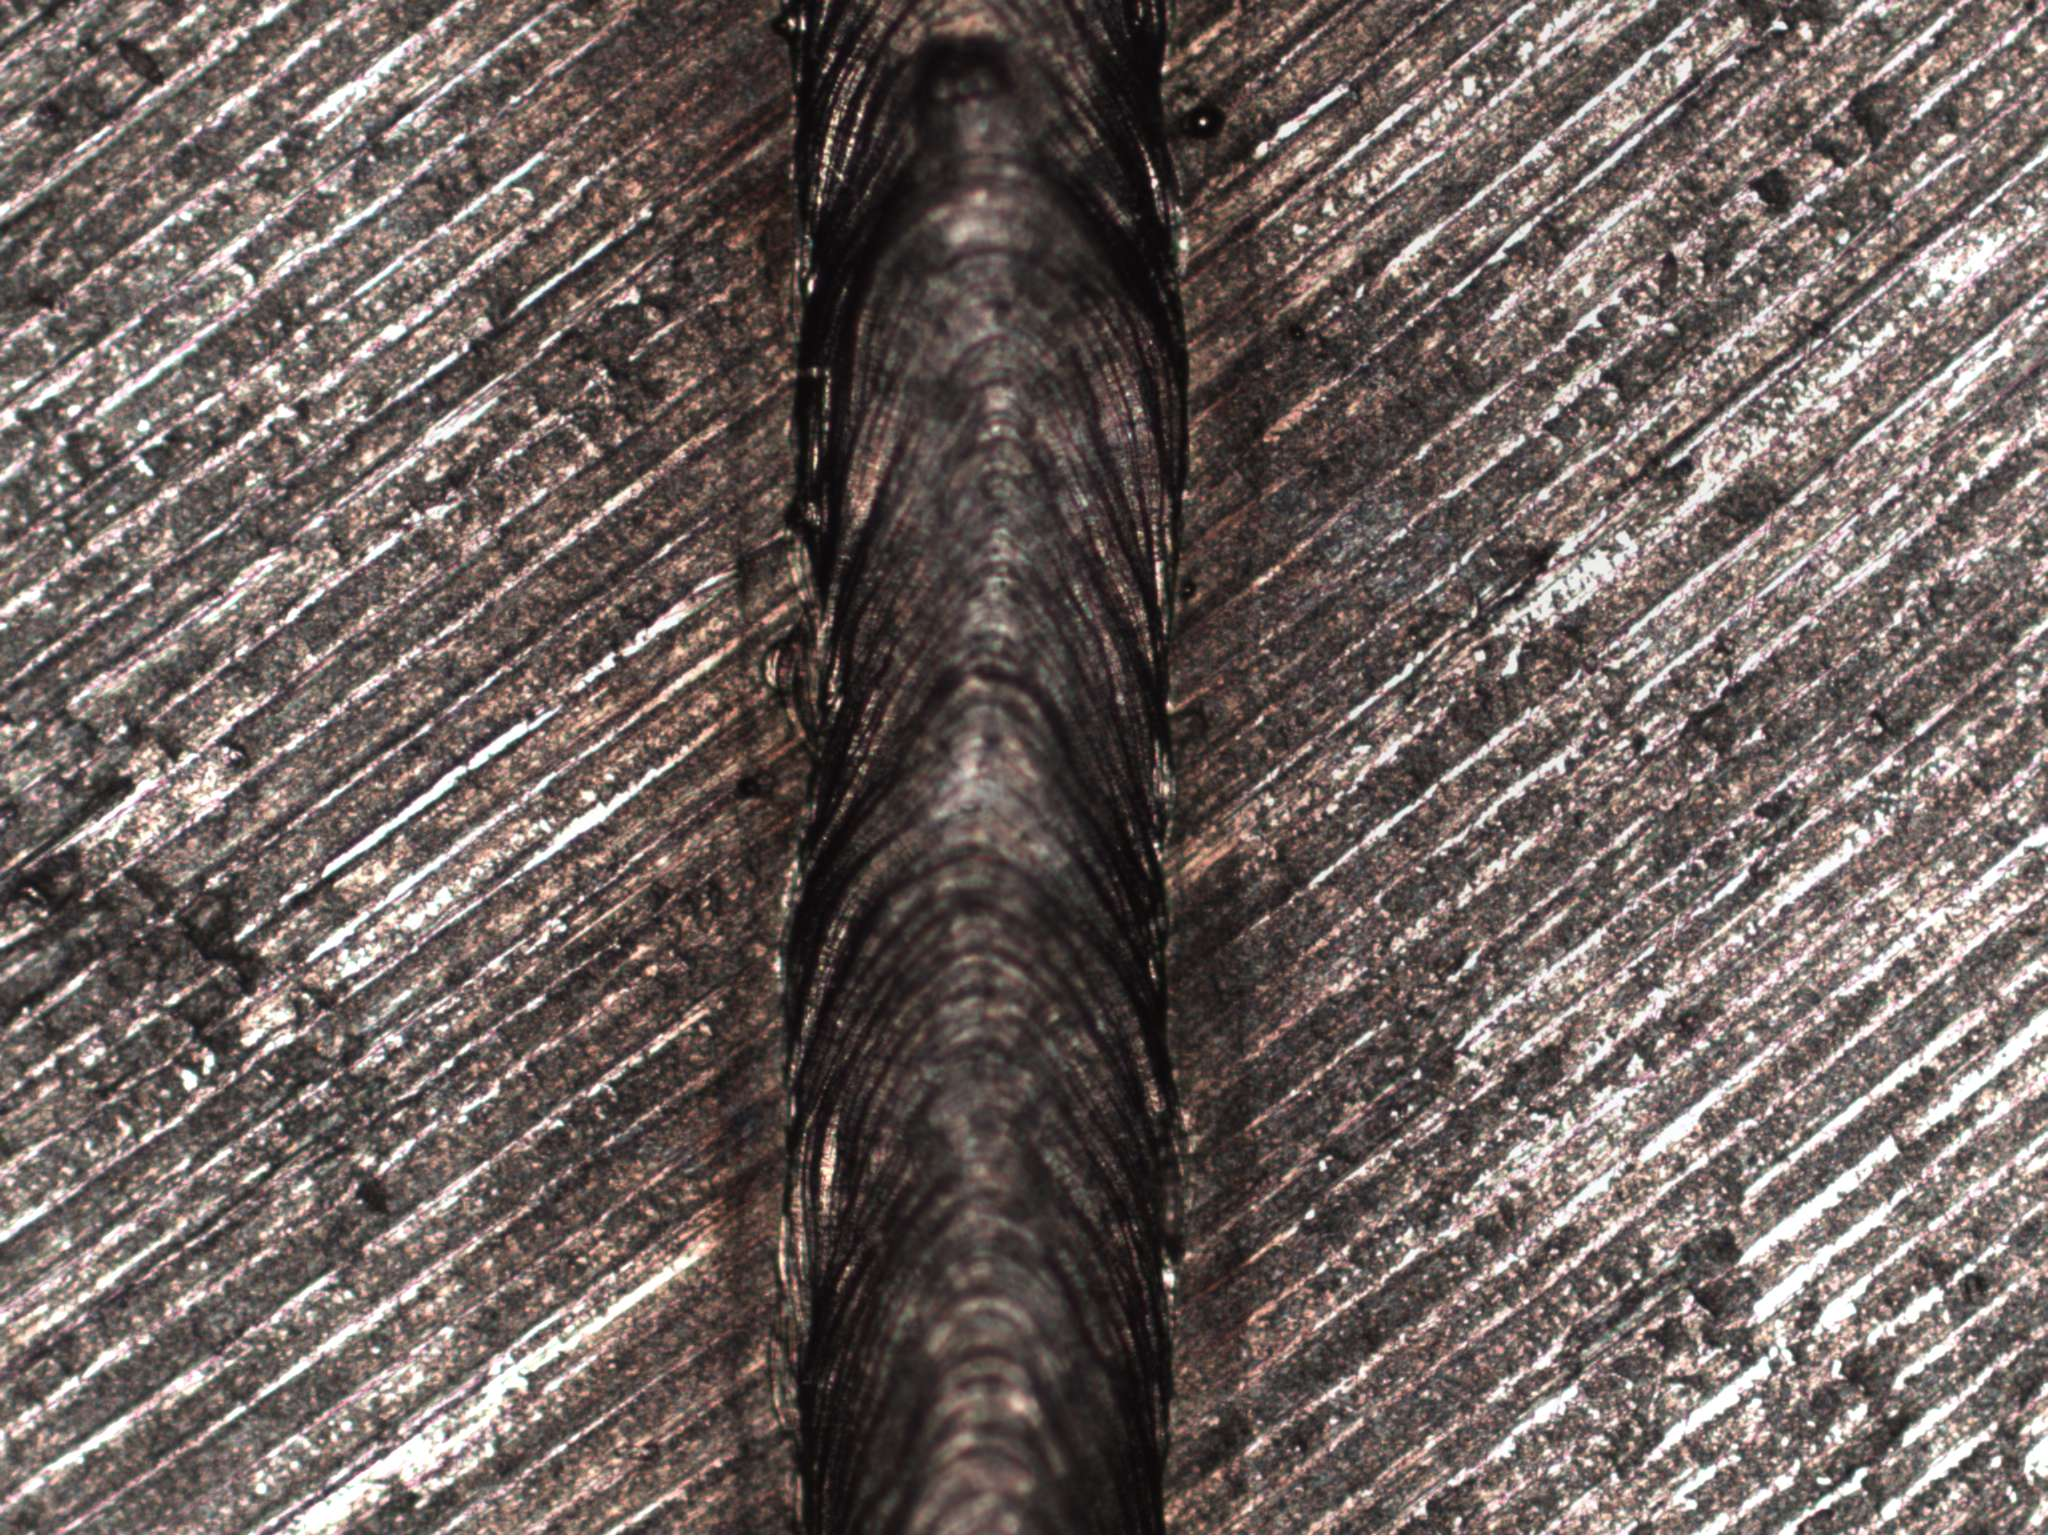
\includegraphics[width=\textwidth]{experiment/photos/90W_V100}
        \caption{\SI{100}{mm/s}}
    \end{subfigure}\:
    \begin{subfigure}[b]{0.24\textwidth}
        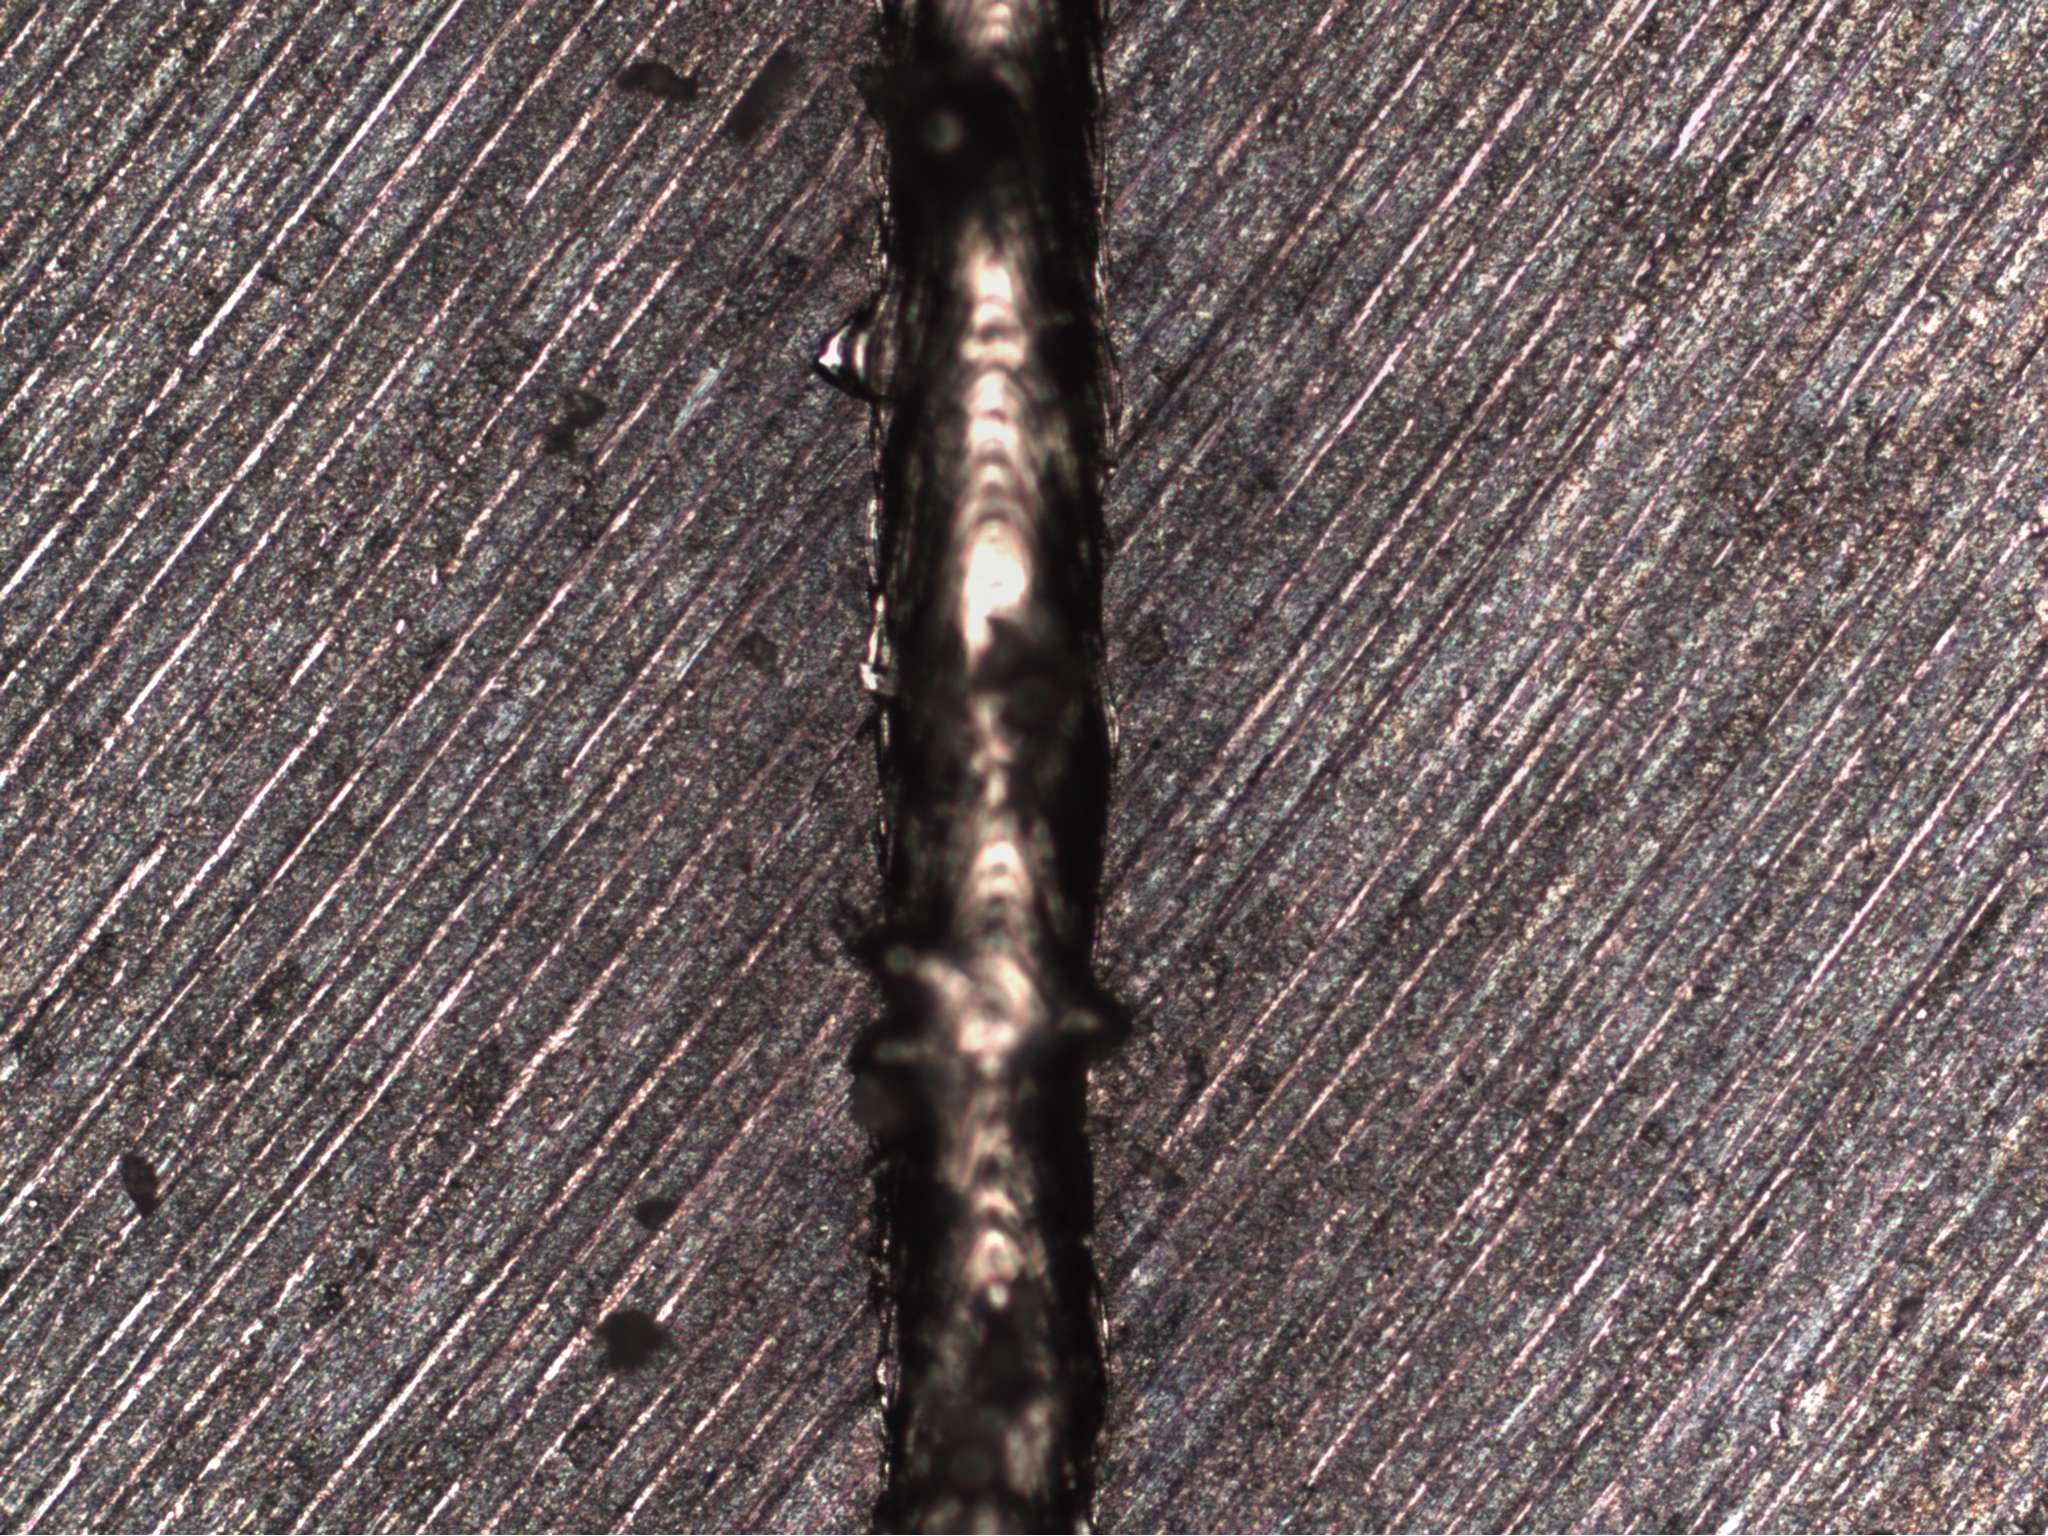
\includegraphics[width=\textwidth]{experiment/photos/90W_V300}
        \caption{\SI{300}{mm/s}}
    \end{subfigure}\:
    \begin{subfigure}[b]{0.24\textwidth}
        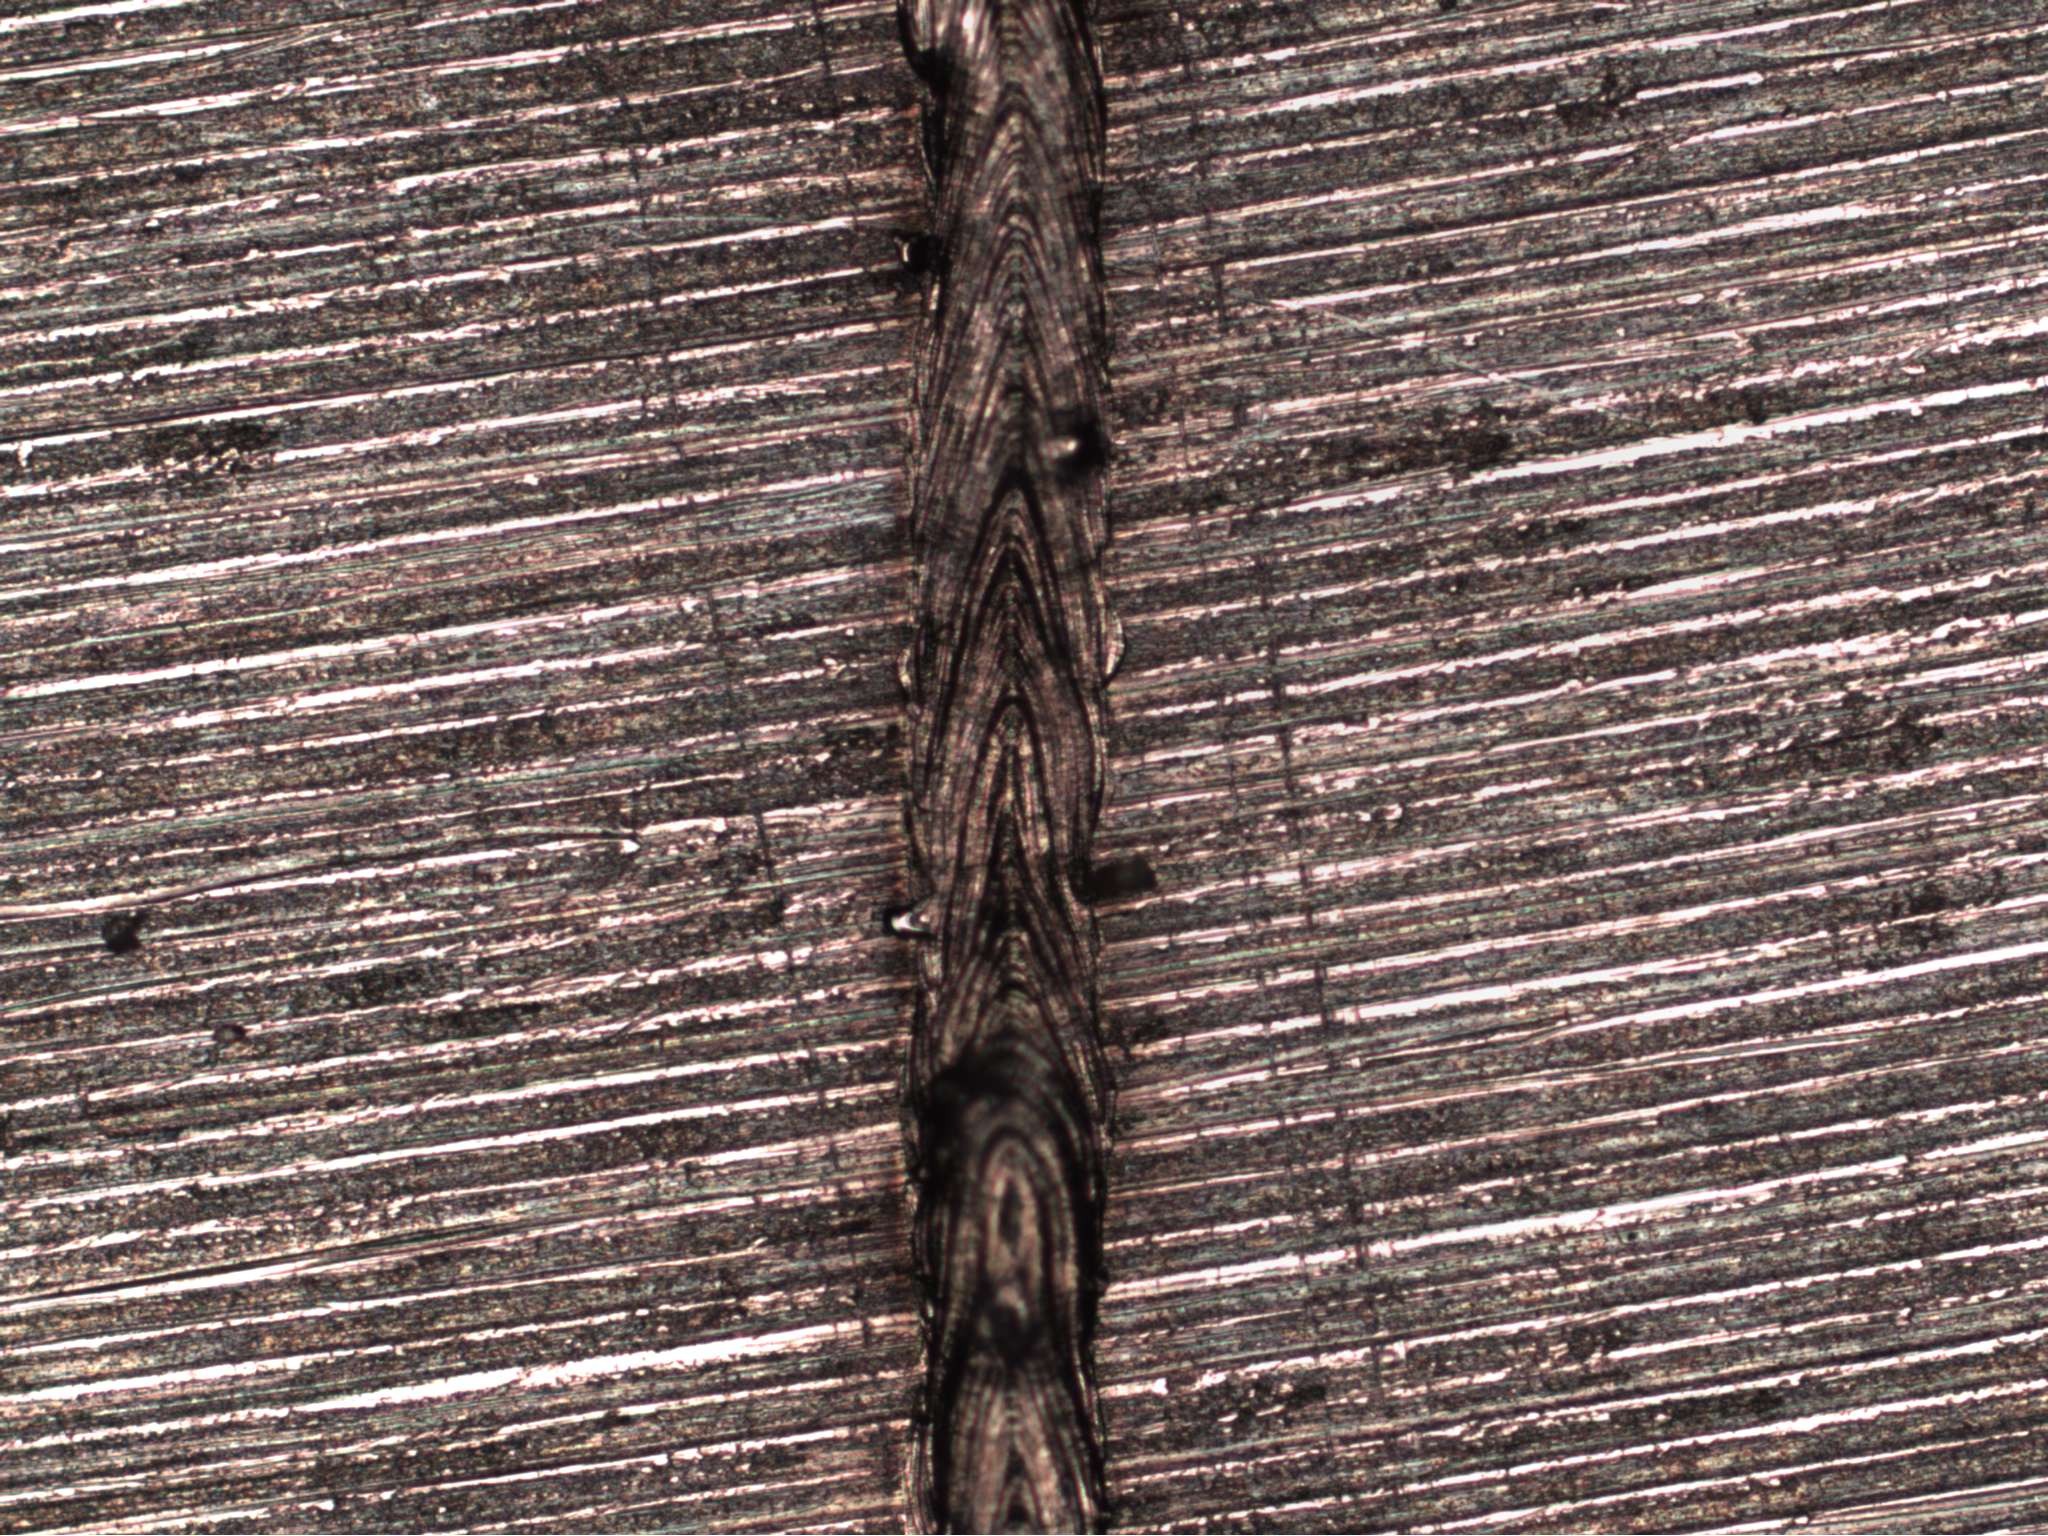
\includegraphics[width=\textwidth]{experiment/photos/90W_V600}
        \caption{\SI{600}{mm/s}}
    \end{subfigure}\:
    \begin{subfigure}[b]{0.24\textwidth}
        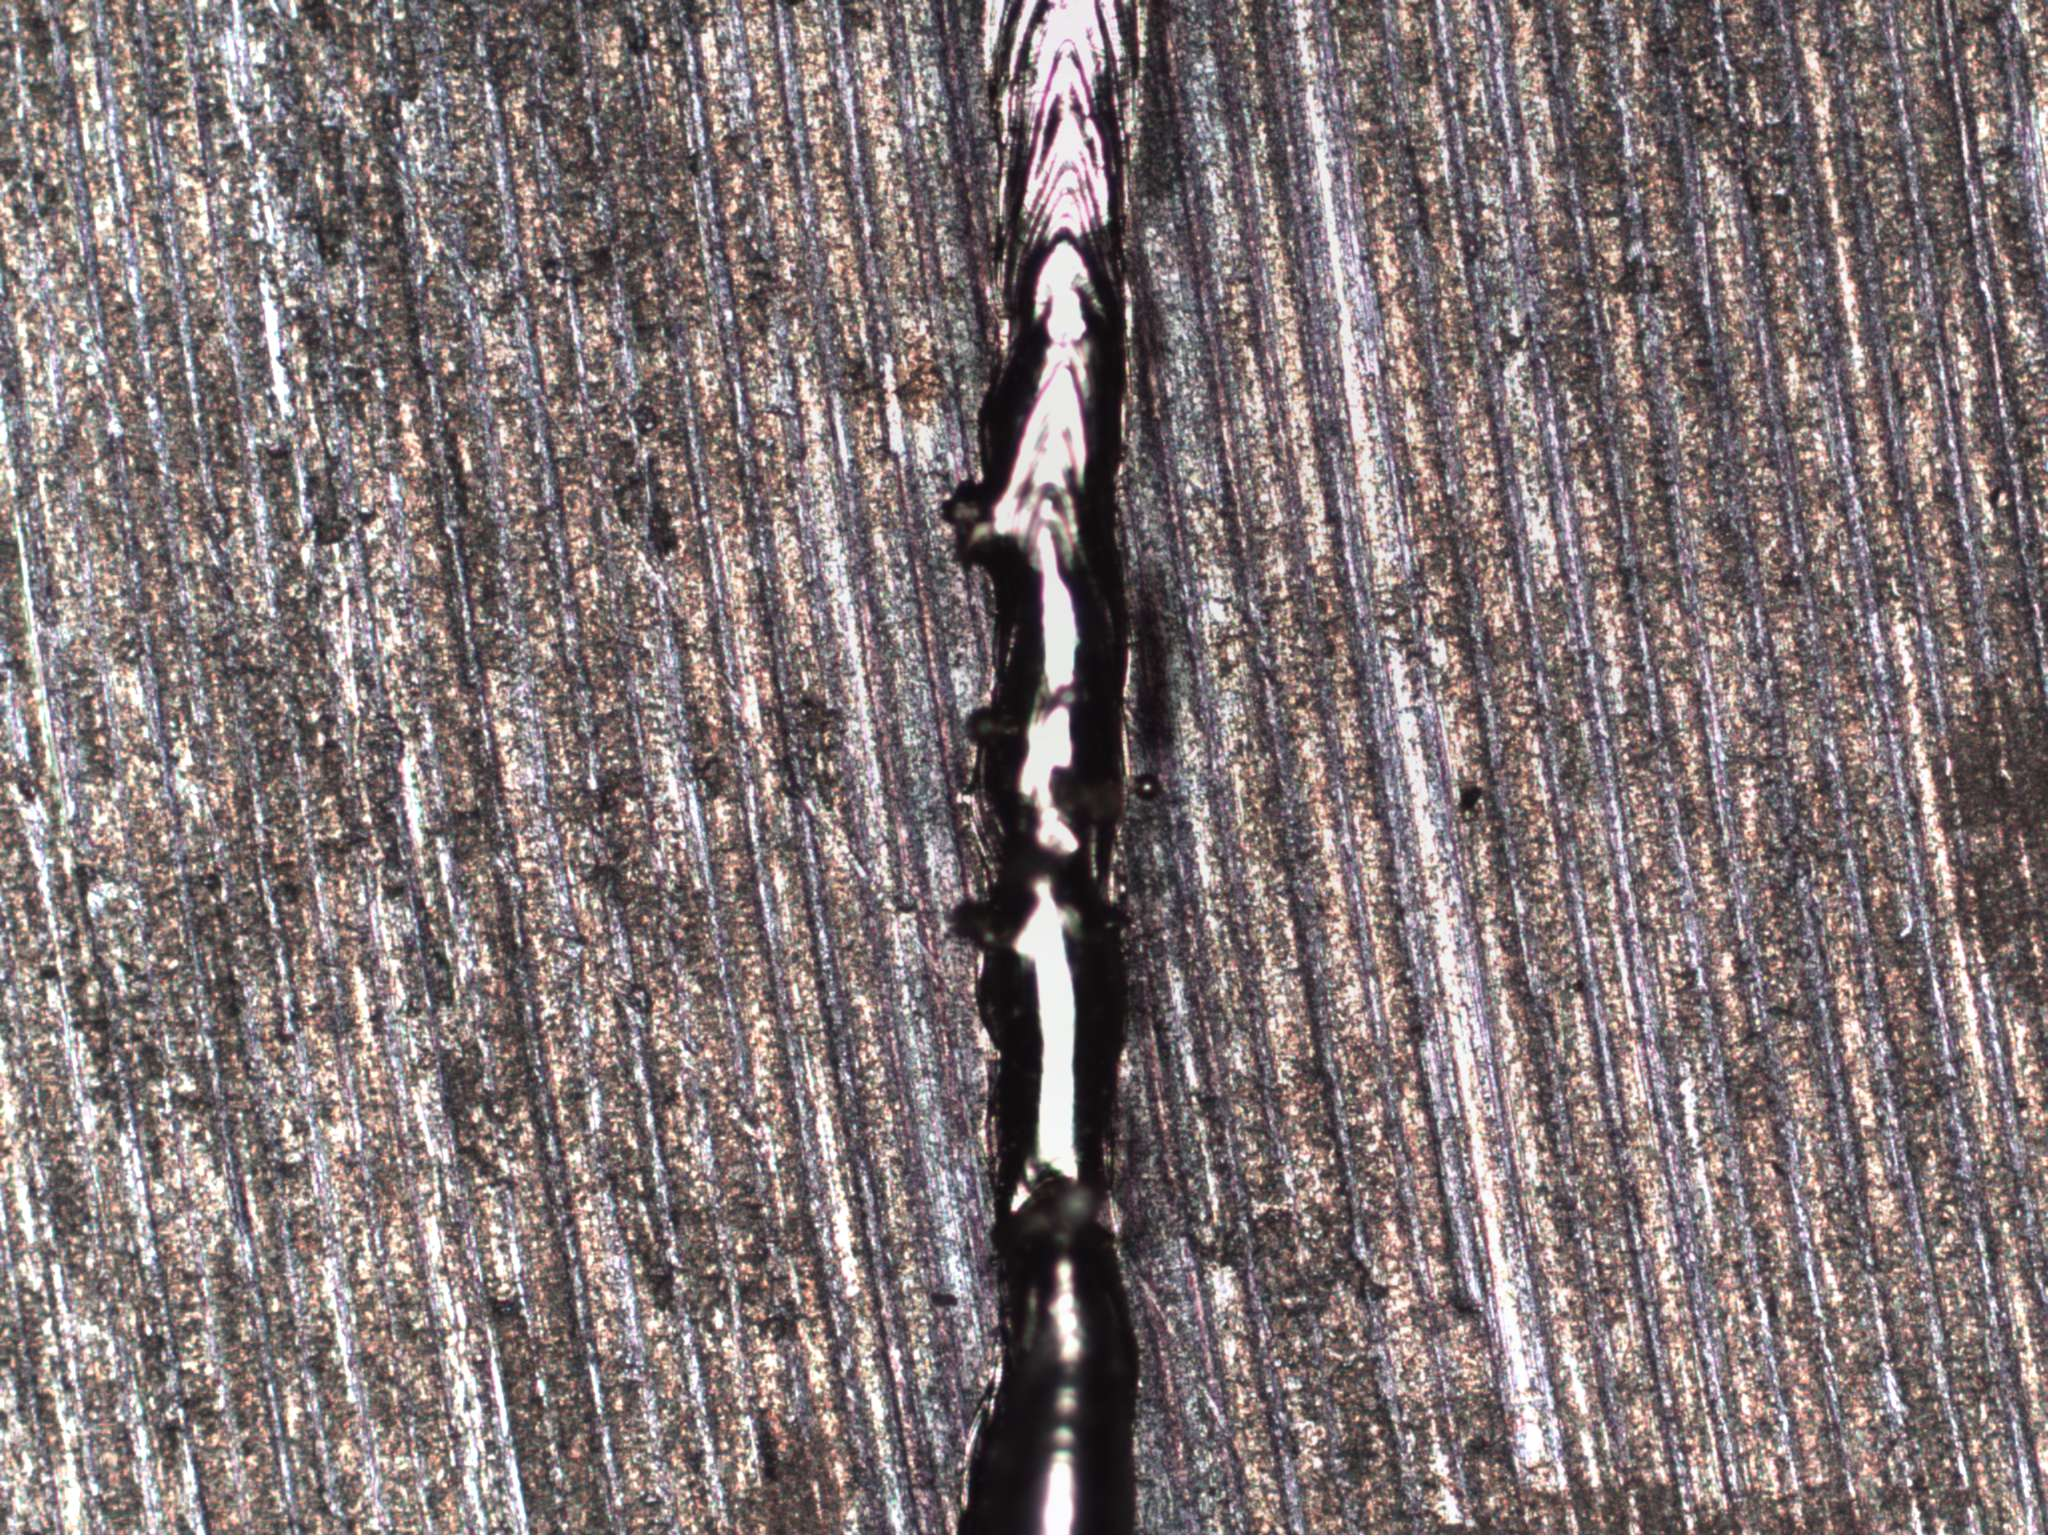
\includegraphics[width=\textwidth]{experiment/photos/90W_V900}
        \caption{\SI{900}{mm/s}}
    \end{subfigure}\\[6pt]
    \begin{subfigure}[b]{0.24\textwidth}
        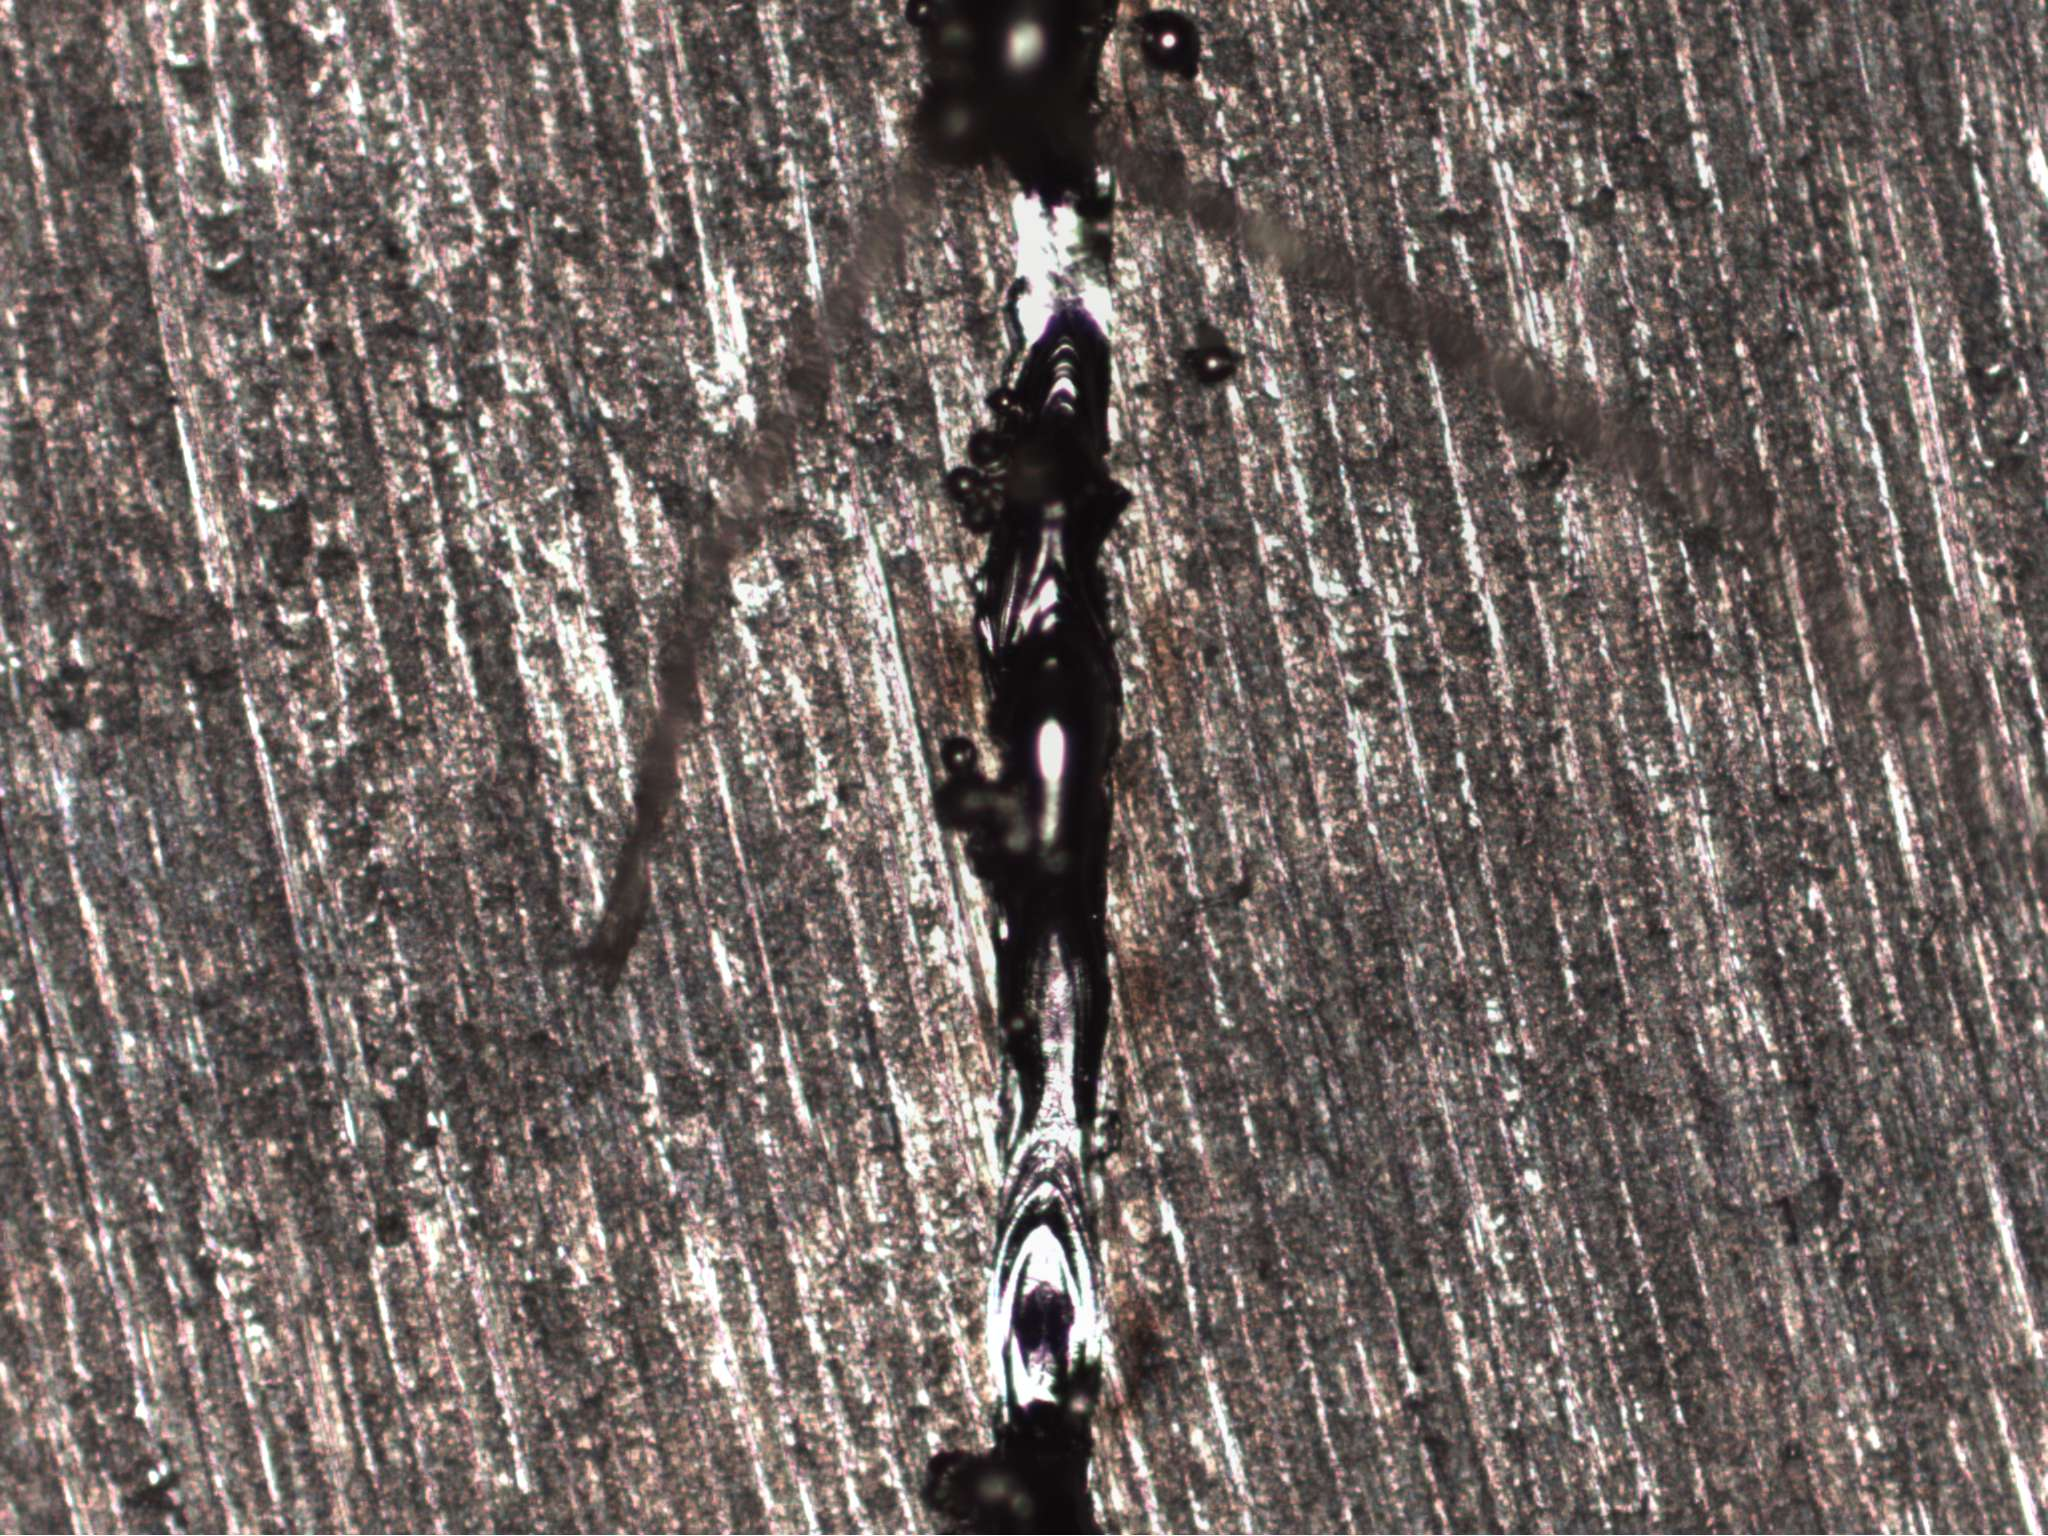
\includegraphics[width=\textwidth]{experiment/photos/90W_V1200}
        \caption{\SI{1200}{mm/s}}
    \end{subfigure}\:
    \begin{subfigure}[b]{0.24\textwidth}
        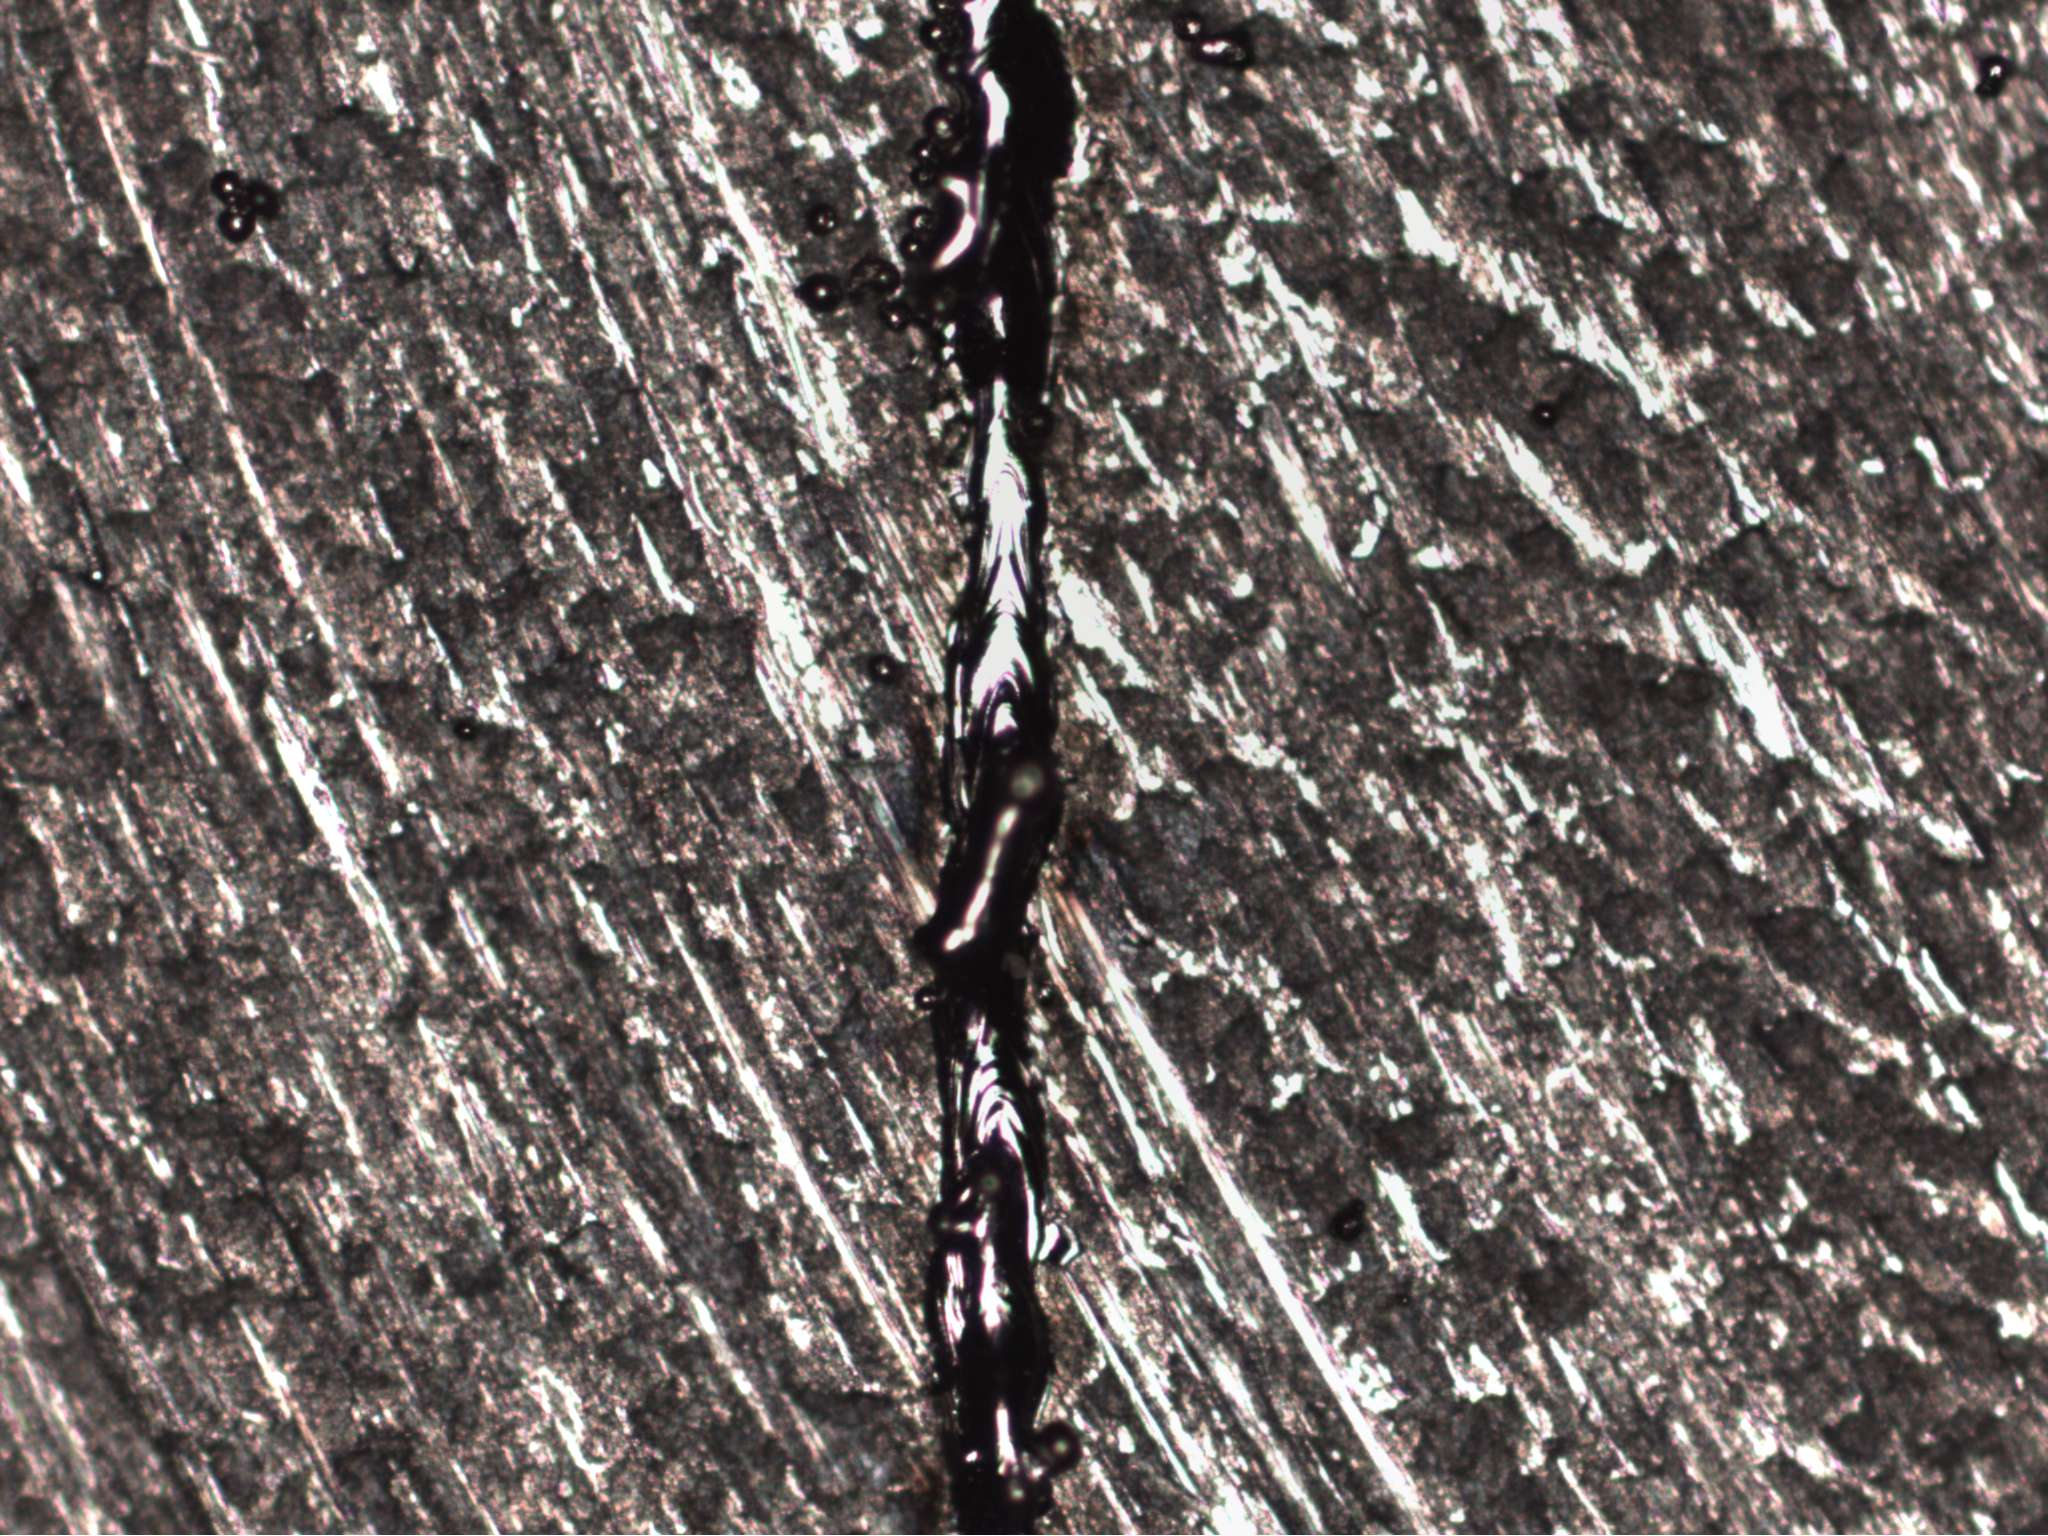
\includegraphics[width=\textwidth]{experiment/photos/90W_V1500}
        \caption{\SI{1500}{mm/s}}
    \end{subfigure}\:
    \begin{subfigure}[b]{0.24\textwidth}
        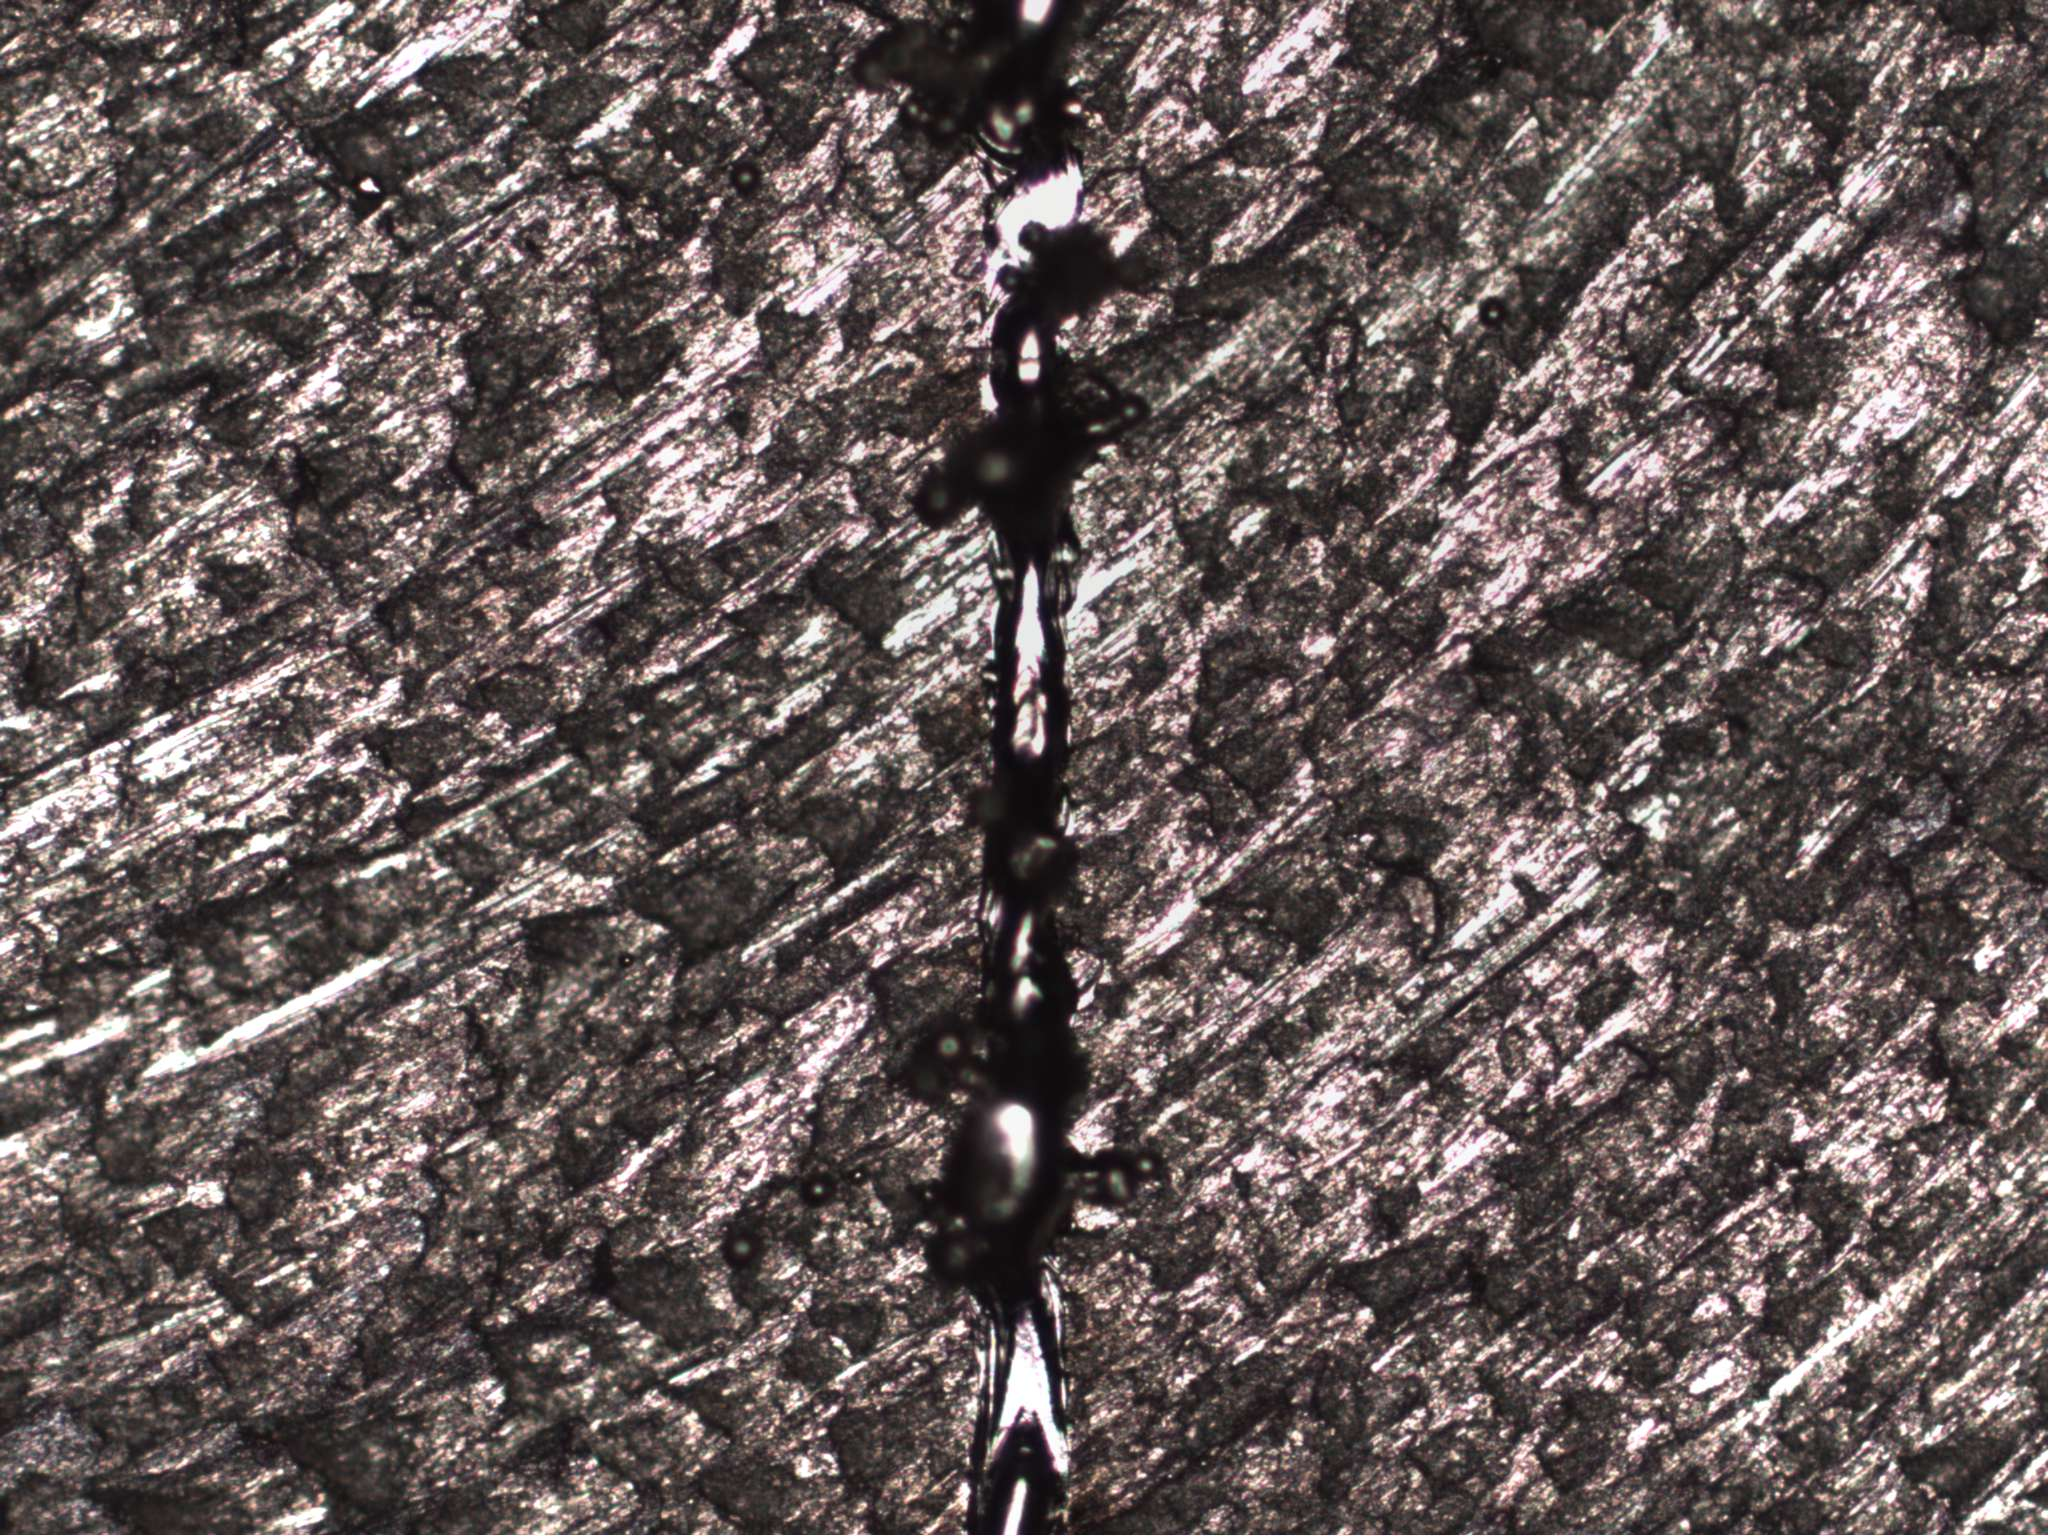
\includegraphics[width=\textwidth]{experiment/photos/90W_V1800}
        \caption{\SI{1800}{mm/s}}
    \end{subfigure}\:
    \begin{subfigure}[b]{0.24\textwidth}
        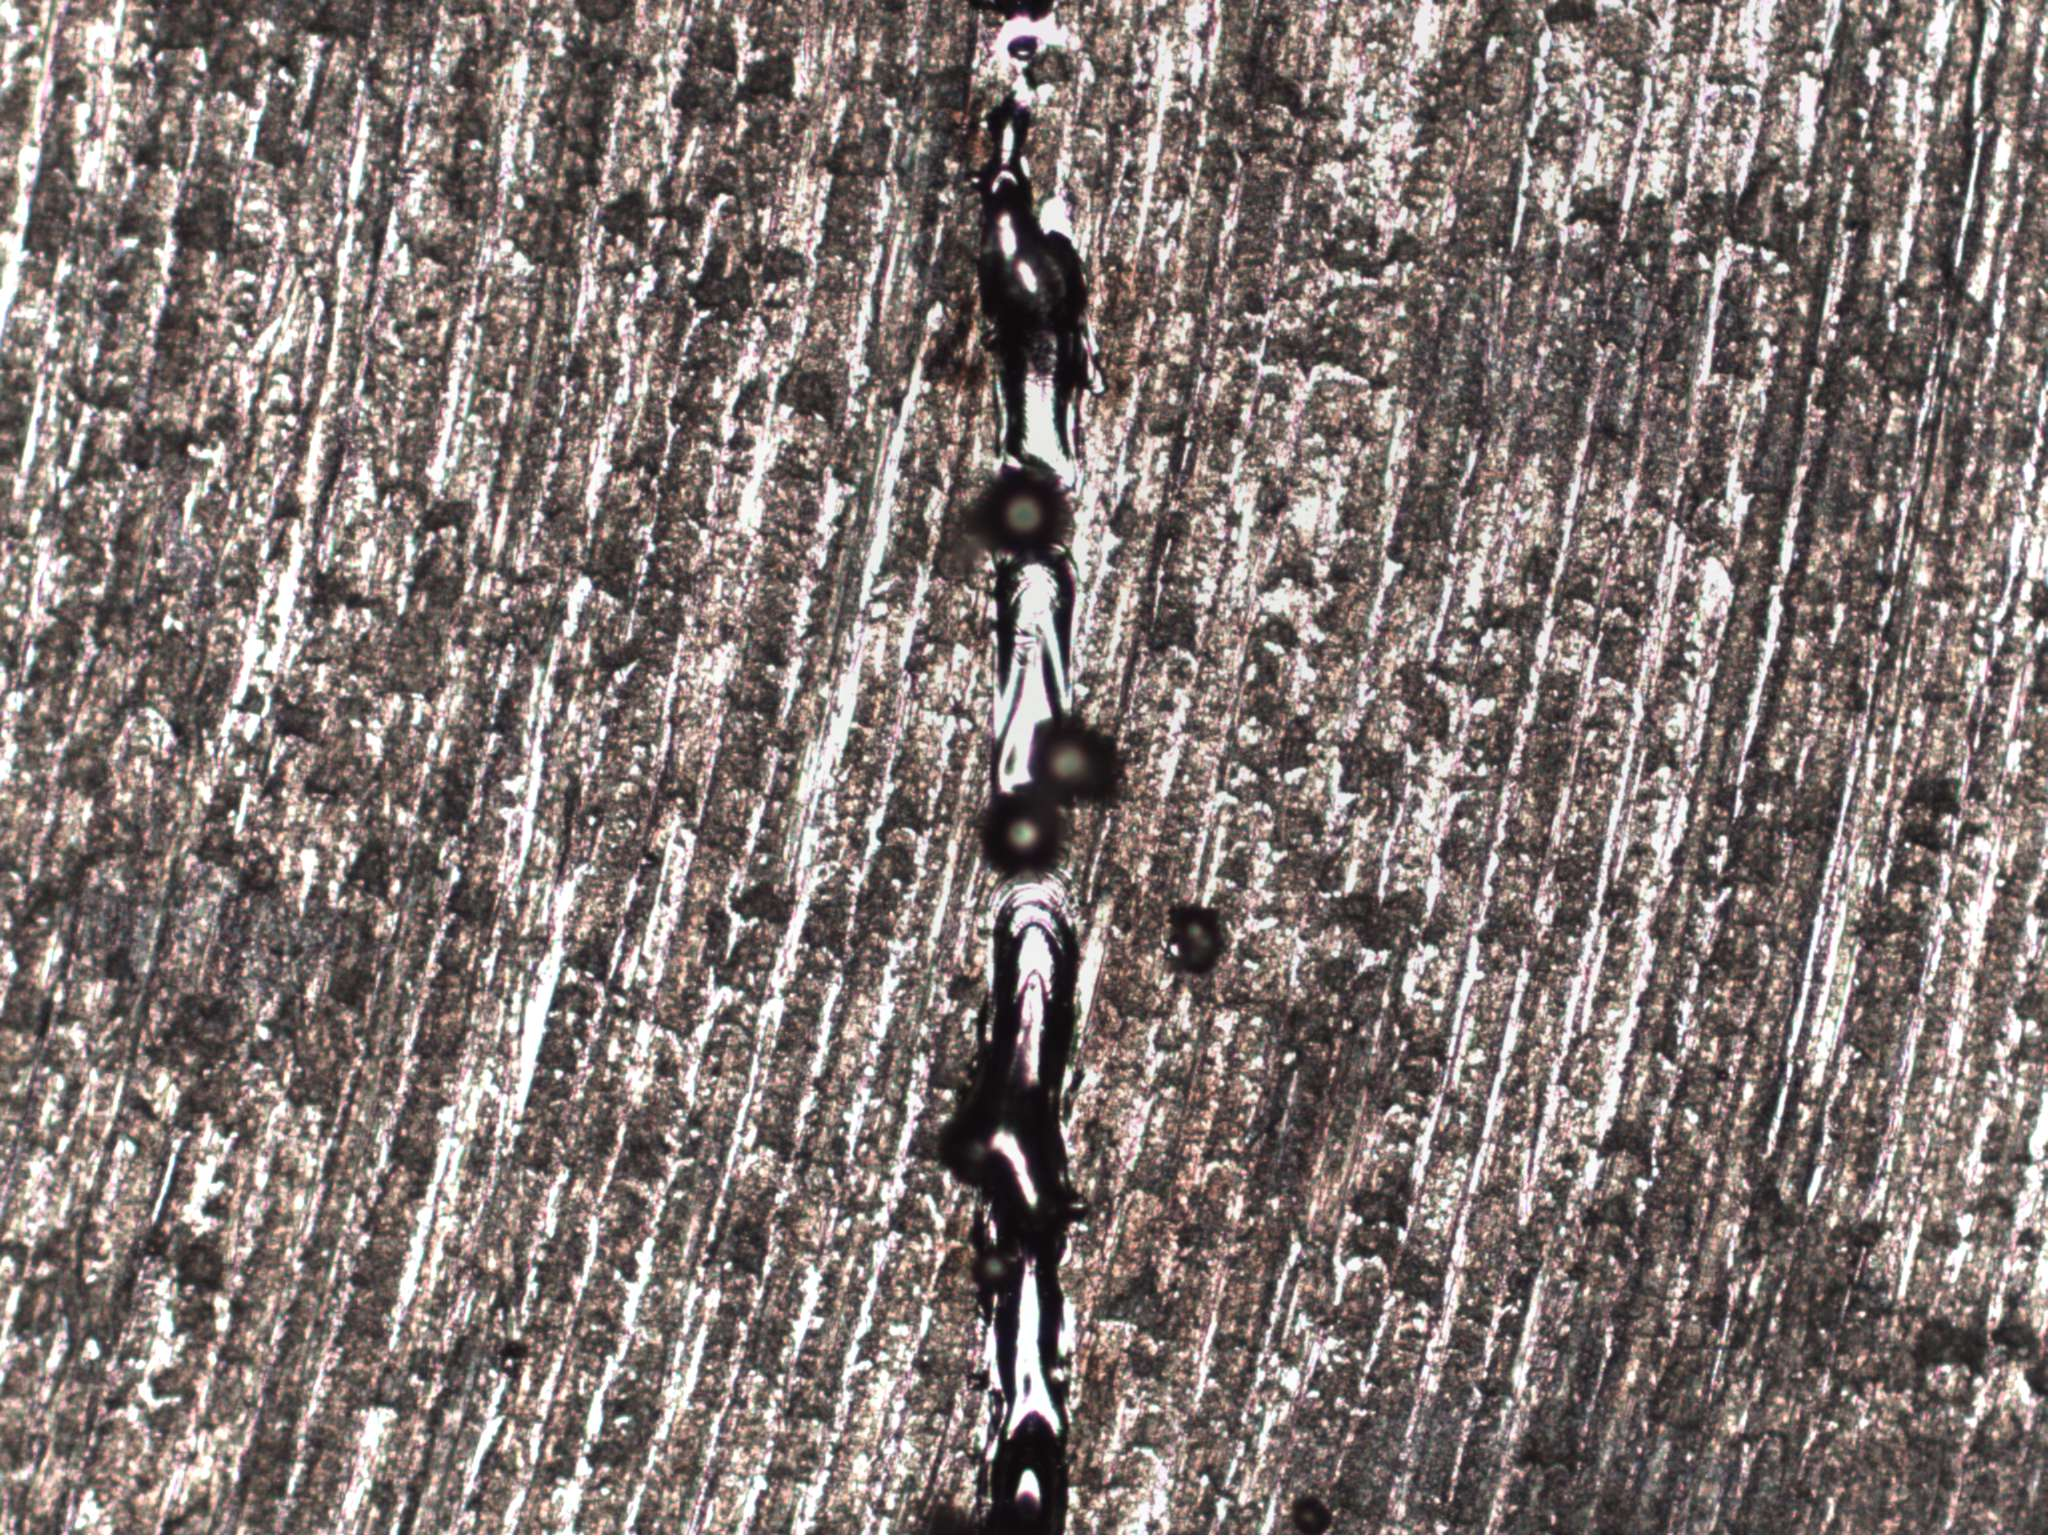
\includegraphics[width=\textwidth]{experiment/photos/90W_V2100}
        \caption{\SI{2100}{mm/s}}
    \end{subfigure}\\[6pt]
    \begin{subfigure}[b]{0.24\textwidth}
        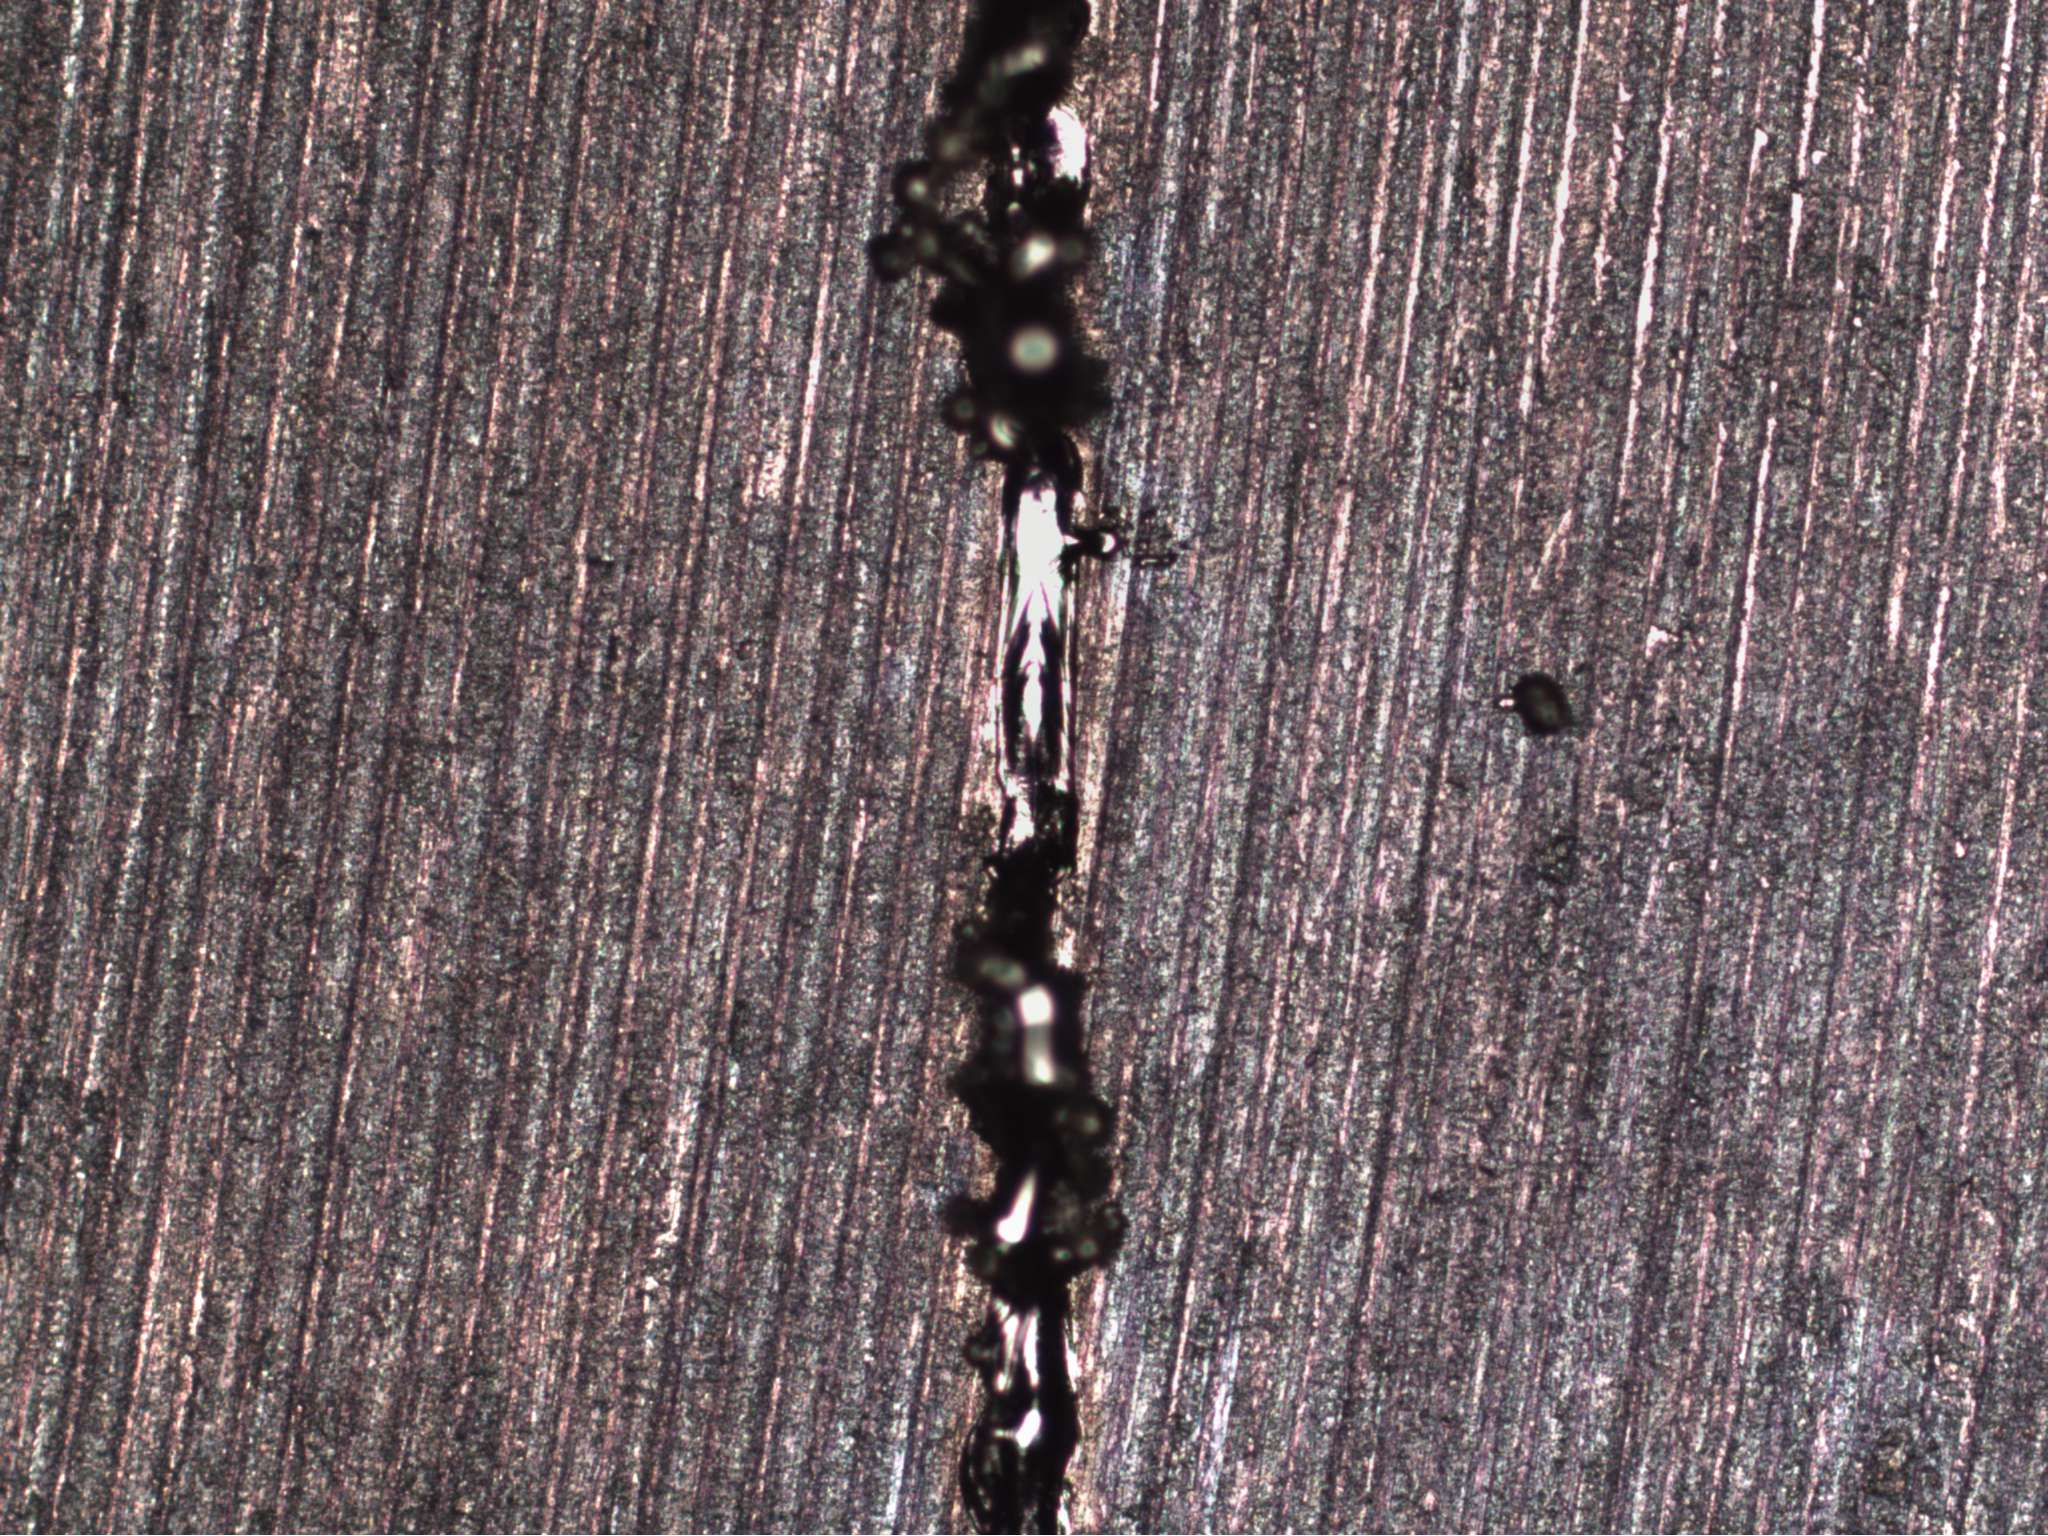
\includegraphics[width=\textwidth]{experiment/photos/90W_V2400}
        \caption{\SI{2400}{mm/s}}
    \end{subfigure}\:
    \begin{subfigure}[b]{0.24\textwidth}
        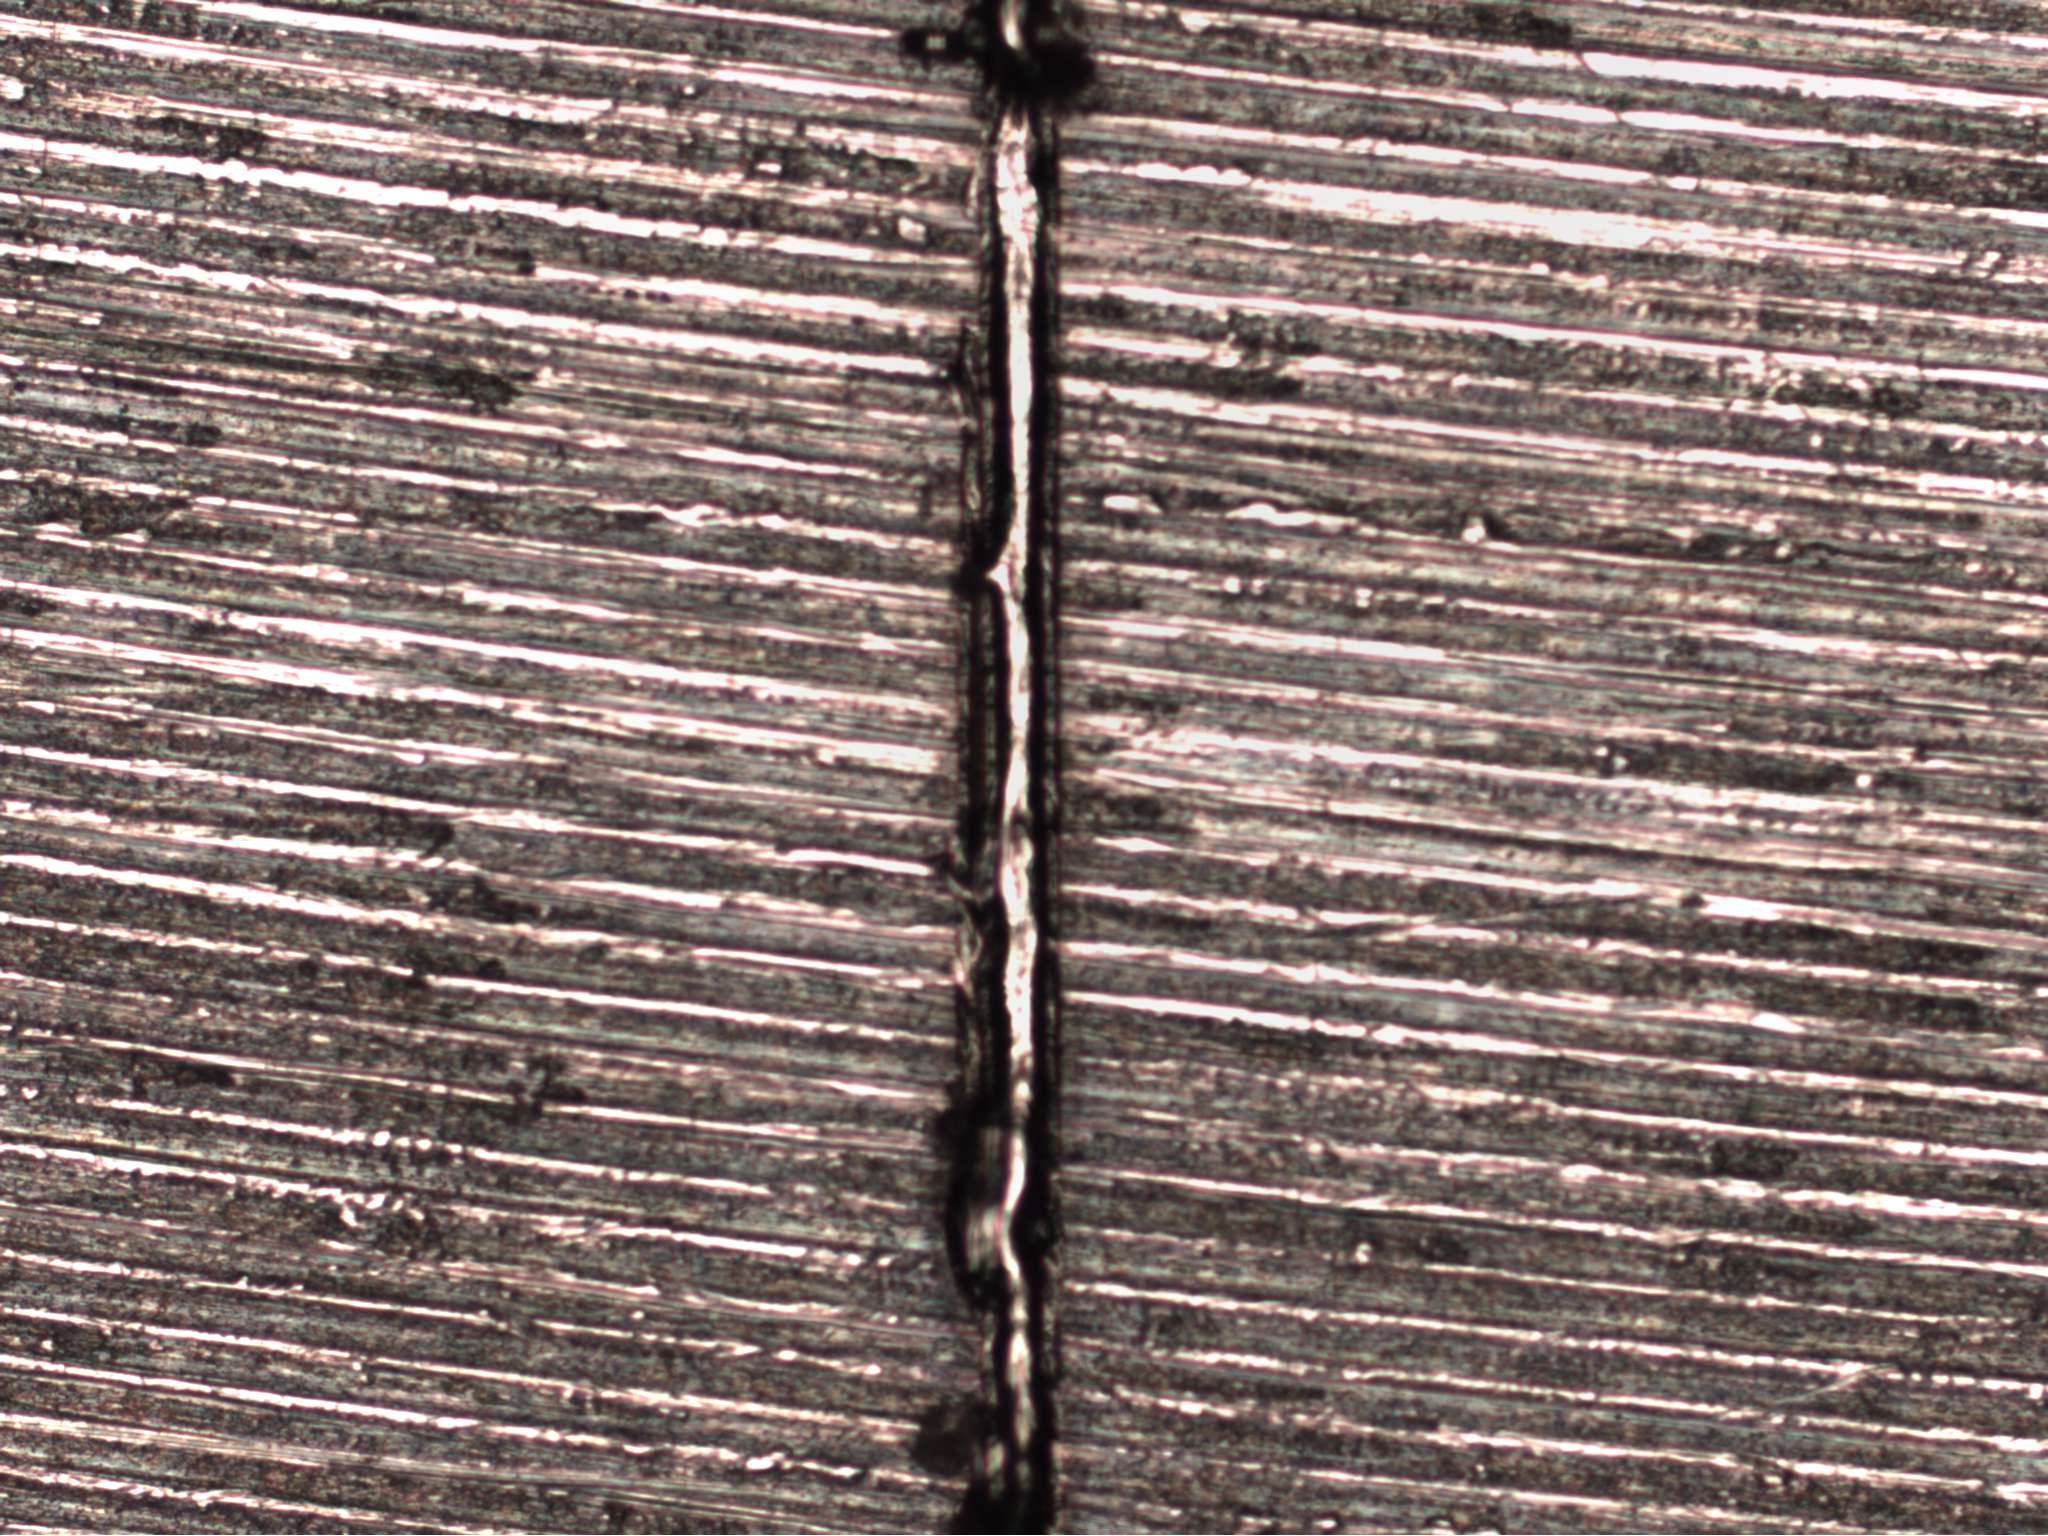
\includegraphics[width=\textwidth]{experiment/photos/90W_V2700}
        \caption{\SI{2700}{mm/s}}
    \end{subfigure}\:
    \begin{subfigure}[b]{0.24\textwidth}
        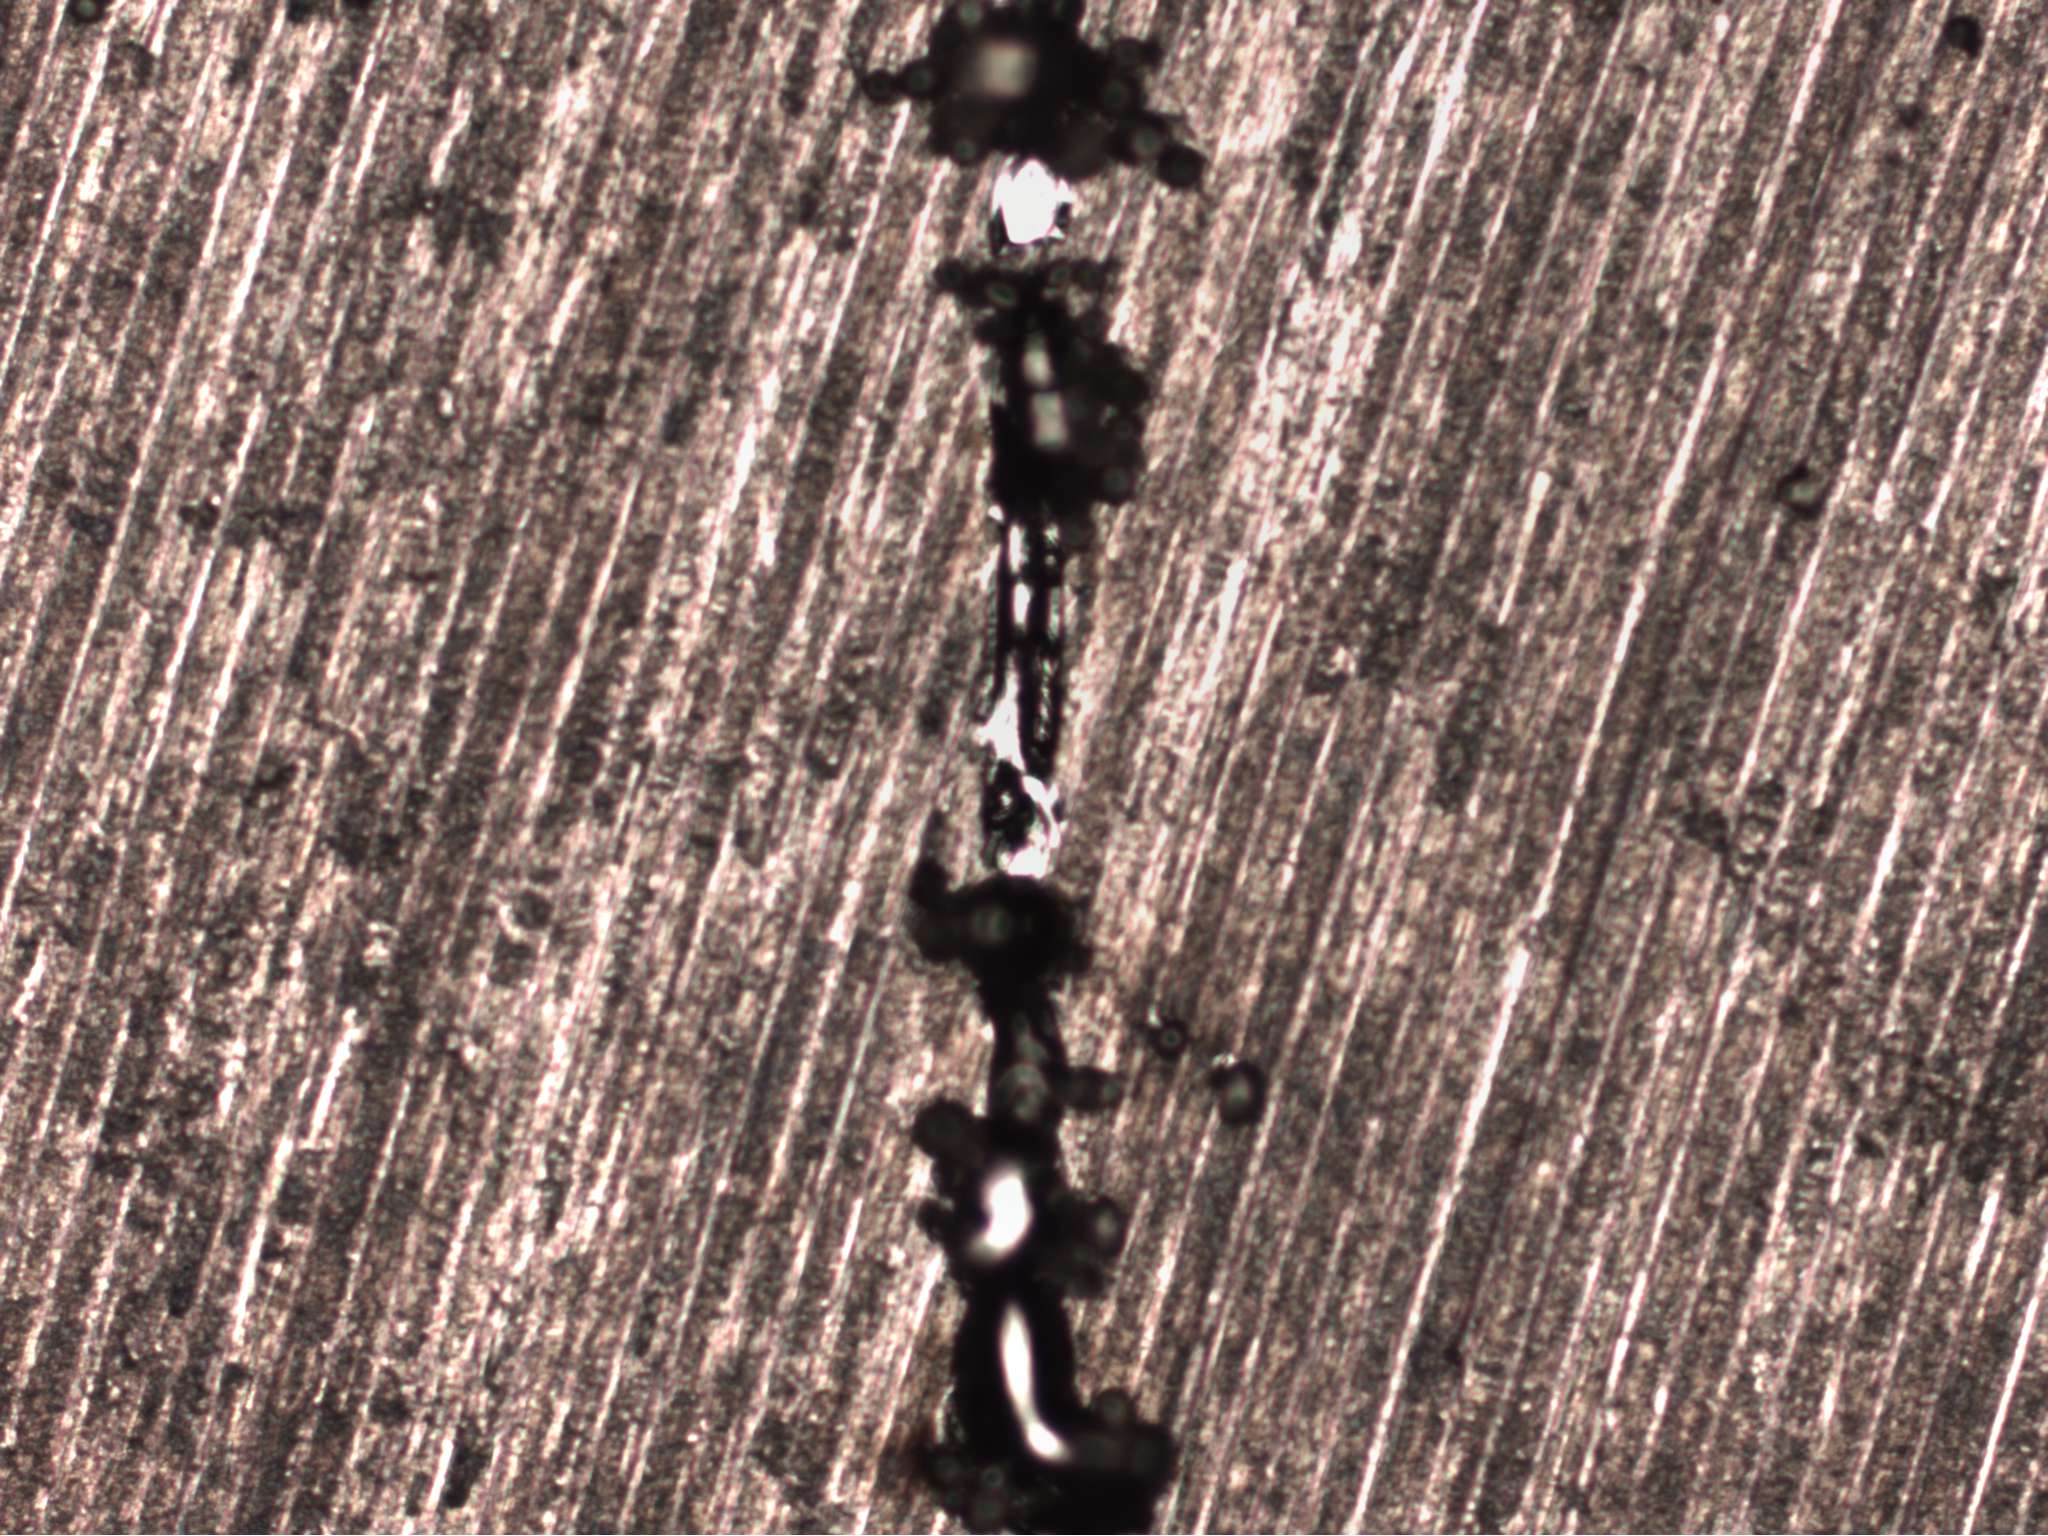
\includegraphics[width=\textwidth]{experiment/photos/90W_V3000}
        \caption{\SI{3000}{mm/s}}
    \end{subfigure}\:
    \begin{subfigure}[b]{0.24\textwidth}
        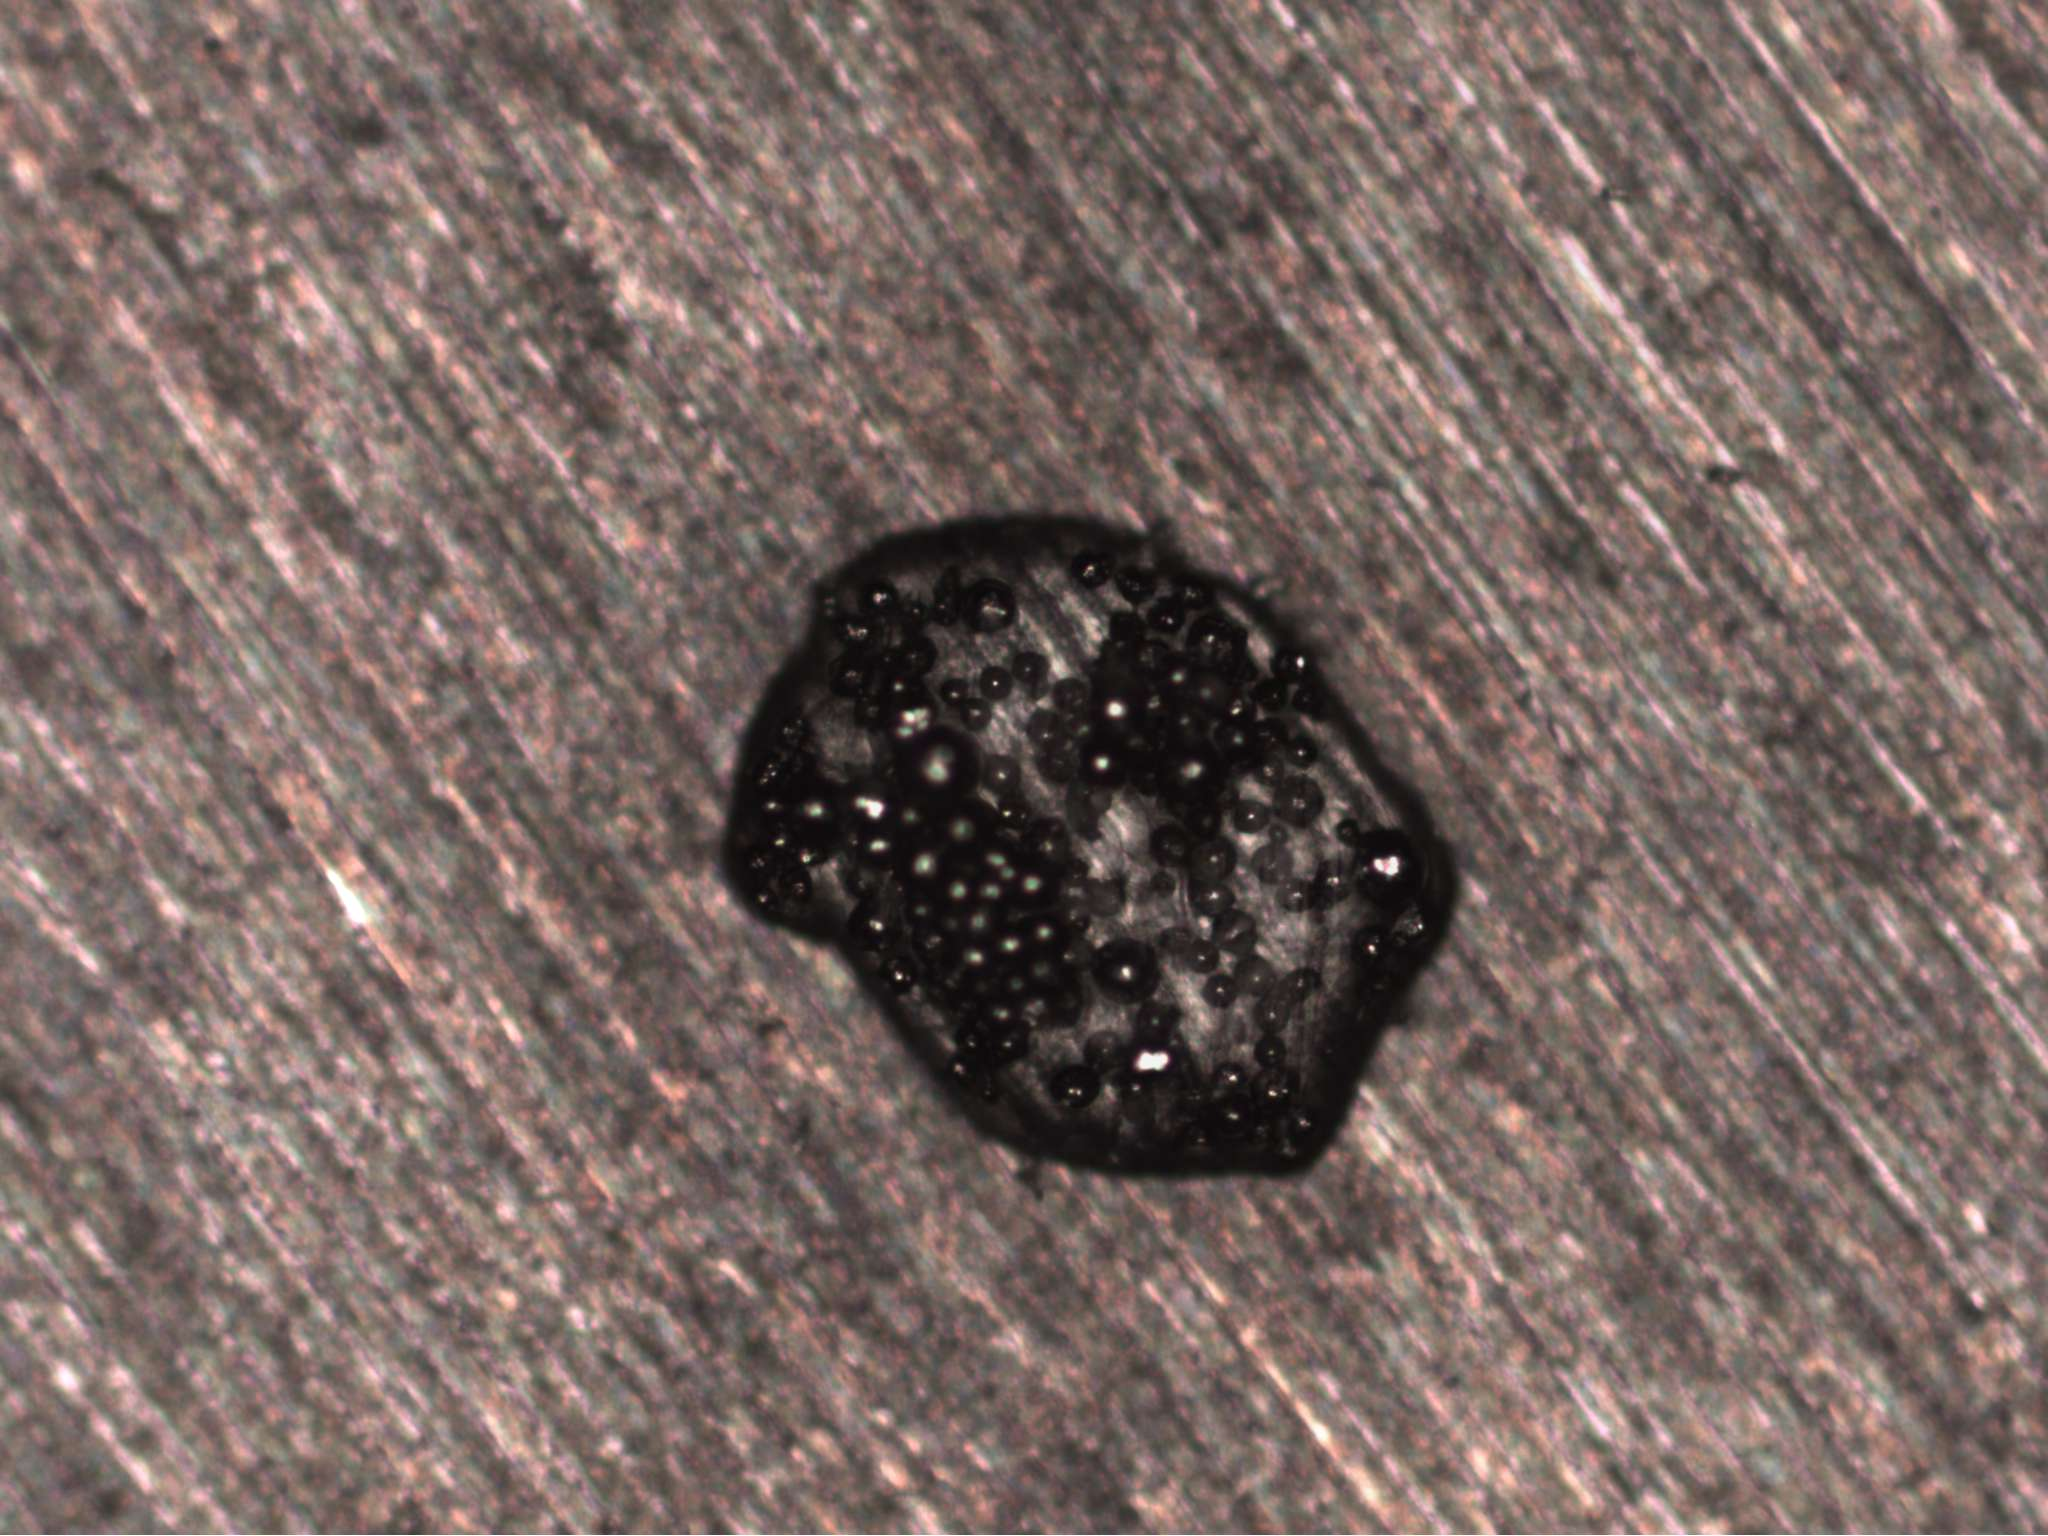
\includegraphics[width=\textwidth]{experiment/photos/powder}
        \caption{powder}
    \end{subfigure}
    \caption{
        Optical microscopy.
        Single tracks after scanning the only powder layer by laser beam
        with \(P=\SI{90}{W}\) and various speeds.
    }
    \label{fig:3d:experiment}
\end{figure}

\begin{figure}
    \centering
    \includegraphics{experiment/width}
    \caption{
        The width of a track versus the scanning speed.
        The solid and dashed lines correspond to the experimental and numerical results, respectively.
    }\label{fig:3d:width}
\end{figure}

\begin{table}
    \centering
    \caption{
        The track width \(d\) in dependence of the laser power \(P\) and scanning speed \(U_0\).
    }\label{table:3d:width}
    \centering
    \begin{tabular}{|c|cccc|ccc|}\hline
        & \multicolumn{4}{c|}{Experimental} & \multicolumn{3}{c|}{Numerical} \\\hline
        \(P\) & \SI{60}{W} & \SI{90}{W} & \SI{120}{W} & \SI{150}{W} & \SI{60}{W} & \SI{90}{W} & \SI{150}{W} \\\hline
        \(U_0\) (\si{mm/s}) & \multicolumn{4}{c|}{\(d\) (\si{\um})} & \multicolumn{3}{c|}{\(d\) (\si{\um})} \\\hline
        100  & 175 & 220 & 245 & 270 &     &     &     \\
        150  &     &     &     &     & 121 & 147 & 183 \\
        300  & 105 & 140 & 145 & 165 & 106 & 129 & 165 \\
        600  & 73  & 110 & 115 & 135 & 91  & 105 & 132 \\
        900  & 65  & 80  & 90  & 110 &     &     &     \\
        1200 & 58  & 70  & 78  & 90  & 73  & 87  & 105 \\
        1500 & 50  & 60  & 70  & 80  &     &     &     \\
        1800 & 46  & 50  & 55  & 72  &     &     &     \\
        2100 & 42  & 45  & 52  & 68  &     &     &     \\
        2400 & 38  & 40  & 52  & 73  & 62  & 74  & 87  \\
        2700 & 33  & 40  & 52  & 70  &     &     &     \\
        3000 & 30  & 36  & 50  & 64  &     &     &     \\\hline
    \end{tabular}
\end{table}

In order to validate the proposed macroscopic model, a number of tracks was printed by Trumpf TruPrint 1000.
Some pictures obtained from the optical microscope are shown in Fig.~\ref{fig:3d:experiment}.
It is seen that too small scanning speed leads to overheating,
but nonuniform and discontinuous tracks are observed for the opposite case.

The current model is unable to describe such instabilities,
but it is possible to compare the resulting track width.
The following parameters are taken to reproduce the mention printing process:
\begin{equation}\label{eq:single:trumpf}
    2R=\SI{55}{\um}, \quad H=\SI{30}{\um}.
\end{equation}
As seen from Fig.~\ref{fig:3d:width} and Tab.~\ref{table:3d:width},
the numerical and experimental results appear to be quite close, especially in the middle regimes (from 300 to 600 \si{mm/s}).
In practice, they correspond to the main operating modes.
Since fluid dynamics and surface tension, along with the powder structure, are not taken into account,
the difference grows for the lowest and highest values of the scanning speed.

\printbibliography

\end{document}
